\chapter{Design}\label{ch:design}
In this chapter we will provide an overview of how the defects in SiC can be used for \index{magnetometry}{magnetometry}, \index{thermometry}{thermometry} and \index{electrometry}{electrometry} in isolation. We will then develop a framework where by combining specific defects we may simultaneously measure multiple parameters. 

% \section{$S=1$ Magnetometry}
We begin by considering a triplet state, that is a $S=1$ system.

Under the influence of a magnetic field, the Hamiltonian can be expressed as:
\begin{equation}
	H_{} = H_{\ce{D}} + H_{\ce{Z}}}
	\label{eq:nv_hamil}
\end{equation}

Here the labels $\ce{D}$ and $\ce{Z}$ describe the electron spin-spin interactions and the Zeeman interaction with an external magnetic field.

They have the following forms:
\begin{eqnarray}
	H_{\ce{D}} &=& D S_z^2 + E(S_x^2 + S_y^2) \label{H_D} \\
	H_{\ce{Z}} &=& g \mu_B \sum_{j}^{x,y,z} B_j \cdot S_j \label{H_Z} \\
\end{eqnarray}

\subsubsection{Spin-Spin Interaction}

The $E$ and $D$ in equation \ref{H_D} represent the fine structure constants of the spin
system, describing the spin-spin interaction and $S_j$ the corresponding spin operators
in x,y and z-direction.

$D$ is non-zero in system with axis of threefold (or other manifold) symmetry.
The definiteness, orientation and magnitude of $D$ is dependent on the specific spin system being studied.

$E$ occurs when there is a distortion of the point group symmetry, for example strain or an $\vec{E}$ field.
Similarly, the value of $E$ is a characteristic of the nature of the distortion and
the specifics of the spin system being studied.

\subsubsection{Zeeman Interaction}

$B_j$ in equation \ref{H_Z} is the magnetic field along the $x$, $y$ and $z$ direction, $g$ is the $g$-factor of the vacancy and $\mu_B$ the Bohr-Magneton.

% It seems often the scaled parameter $g\mu_B$ is considered, for the $\ce{NV^-}$ system this is around $28\;\ce{ GHz T^{-1}}$, but again, will be a characteristic of the system being studied. 

% \subsubsection{Reduced Hamiltonian}
By combining $H_{\ce{D}}$ and $H_{\ce{Z}}$
we find
\begin{equation}
	H_{} = D S_z^2 + E(S_x^2 + S_y^2) + g \mu_B \sum_{j}^{x,y,z} B_j \cdot S_j
	\label{eq:reduced_H_NV}
\end{equation}

the $S=1$ spin operators \eqref{eq:s1_spin_operators}, then aligning the magnetic field (with strength $B_0$) along the $z$-axis (the quantisation axis), the reduced Hamiltonian will have the form
\begin{equation}
	H_{} = \begin{pmatrix}
		D + B_0 & 0 & E     \\
		0       & 0 & 0     \\
		E       & 0 & D-B_0
	\end{pmatrix},
	\label{eq:reduced_H_NV_matrix}
\end{equation}

with Eigenvalues

\begin{equation}
	E_x = E_y = D \pm \sqrt{B_0^2  + E^2}, \; E_z = 0.
	\label{eq:reduced_H_NV_eigenvalues}
\end{equation}

The corresponding non-normalised Eigenvectors are then

\begin{eqnarray}
	\ket{X} = \frac{1}{E} \left(B_0 + \sqrt{B_0^2 + E^2}\right) \ket{+1} + \ket{-1} \\
	\ket{Y} = \frac{1}{E} \left(B_0 - \sqrt{B_0^2 + E^2}\right) \ket{+1} + \ket{-1} \\
	\ket{Z} = \ket{0},
\end{eqnarray}
with
\begin{equation}
	\ket{1} = \begin{pmatrix}
		1 & 0 & 0
	\end{pmatrix}, \;
	\ket{0} = \begin{pmatrix}
		0 & 1 & 0
	\end{pmatrix}\;,
	\ket{-1} = \begin{pmatrix}
		0 & 0 & 1
	\end{pmatrix},
	\label{eq:base_states}
\end{equation}
the Eigenvectors for $H$ with $E=0$ \td{Need to finish write up. }.

In the case where $E \ll B_0$ the Eigenvectors are well described by the bases $\ket{0}$ and $\ket{\pm 1}$.

For an arbitrary external magnetic field, $H$ can be expressed using spherical co-ordinates:
\begin{equation}
	H = \begin{pmatrix}
		D + B_0 \cdot \cos \theta                                       & \frac{B_0}{\sqrt{2}} \cdot e^{-i\cdot \varphi} \cdot \sin\theta & E                                                         \\
		\frac{B_0}{\sqrt{2}} \cdot e^{i \cdot \varphi} \cdot \sin\theta & 0                                                               & \frac{B_0}{\sqrt{2}} e^{-i\cdot \varphi} \cdot \sin\theta \\
		E                                                               & \frac{B_0}{\sqrt{2}} \cdot e^{i \cdot \varphi} \cdot \sin\theta & D - B_0 \cdot \cos \theta
	\end{pmatrix}
	\label{eq:nv_hamil_spherical_matrix}
\end{equation}


Here, we transformed the magnitude of the arbitrary magnetic field into spherical co-ordinates as
\begin{eqnarray}
	B_x  &=& B_0 \cos\varphi \sin\theta \\
	B_y  &=& B_0 \sin\varphi \sin\theta \\
	B_z  &=& B_0 \cos\theta
\end{eqnarray}
with $\theta$ the azimuthal and $\varphi$ the polar angle. Then using equations \ref{eq:reduced_H_NV} and \ref{eq:spin_operators} we compute \ref{eq:nv_hamil_spherical_matrix}.

It immediately follows from the characteristic \td{need to finish writing this} equation that Eigenvalues $\lambda$ satisfy
\begin{equation}
	0 = \lambda^3 - 2\cdot \lambda^2 \cdot D + \frac{D \cdot B_0^2}{2} + \lambda(D^2 - E^2 - B_0^2) - \frac{1}{2}B_0^2\underbrace{\left(D \cdot \cos(2\theta) - 2 \cdot E \cos(2\varphi) \cdot \sin(\theta)^2\right)}_{\Delta_{\varphi \theta}}
	\label{eq:nv_spherical_characteristic_equation}
\end{equation}
% \cite{balasubramanian2009}




% https://magnetometryrp.quantumtinkerer.tudelft.nl/3_NVspin/


\subsection{$\vec{B}$ Parallel to Defect Axis}
The simplest implementation of the magnetometer is when the applied magnetic field, $B_0$ is parallel to the defect axis.

In this case, the entire magnitude of the field contributes to the Zeeman splitting of the energy level. This means in the CW-ODMR spectra the difference between the two frequencies $f_1 > f_2$ is directly proportional to $B_0$ and related as detailed in Section \ref{zeeman}.
$$f_1 = D + \gamma B_0,  \quad f_2 = D - \gamma B_0$$
It is then straightforward to calculate $B_0$ using
\begin{equation}
	B_0 = \frac{f_1 - f_2}{2 \gamma}
	\label{eq:s1_parallel_magnetometry}
\end{equation}
which is visualised for the DNV system in figure \ref{fig:spin1_magnetometry}.
% \begin{wrapfigure}{r}{0.5\textwidth}%
%     \centering%
%     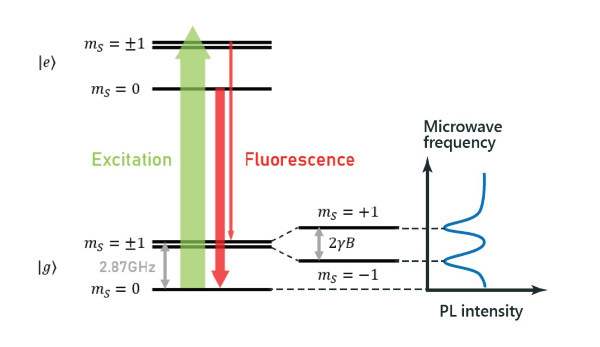
\includegraphics[width=0.5\textwidth]{figures/NVlevelwithESR.png}
%     % 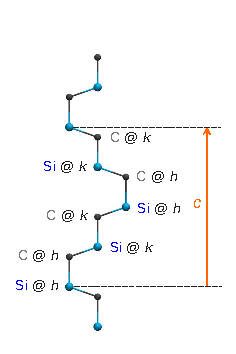
\includegraphics[width=0.38\textwidth]{figures/SiC-non-equiv-sites.pdf}%
%   \caption{Magnetometry with $\theta = 0$. Left shows the lifting of degeneracy of the spin system energy levels with the applied $\vec{B}$ field. Right shows the corresponding ODMR spectra and two EPR frequencies \cite{dnvweb}. \td{better caption}}%
% \label{fig:spin1_magnetometry}
% \end{wrapfigure}

\begin{figure}[h]
	\begin{center}
		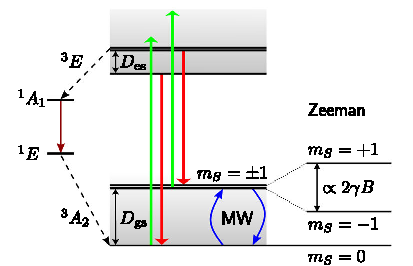
\includegraphics[width=0.7\textwidth]{figures/DNV-ODMR.pdf}
		% \missingfigure{Two panel figure. Panel 1 - energy level splitting of S=1 system being prop to gyromagnetic ratio. Panel 2 - ODMR Spectra} 
	\end{center}
	\caption{ODMR Magnetometry with $\theta = 0$. Degeneracy of the spin system energy levels is lifted with the applied $\vec{B}$ field \cite{Strner2021}. }
	\label{fig:spin1_magnetometry}
\end{figure}
%

\subsubsection{$\vec{B}$ at Angle $\theta$ to Defect Axis}
The Zeeman effect is proportional to $\cos\theta$, thus, when $\vec{B}$ is perpendicular to the defect axis the Zeeman effect reduces to zero, varying the azimuthal angle $\theta$ is effectively the same as scaling $B_0$ by $\cos \theta$.

\td{Reference how this reduction to zero can be exploited in electometry?}

\begin{figure}[h]
	\begin{center}
		% /        \missingfigure{ODMR or Energy Eigenvalues plot for $\theta = 0, 30, 60, 90$ showing the effective reduction of applied parallel field.}
		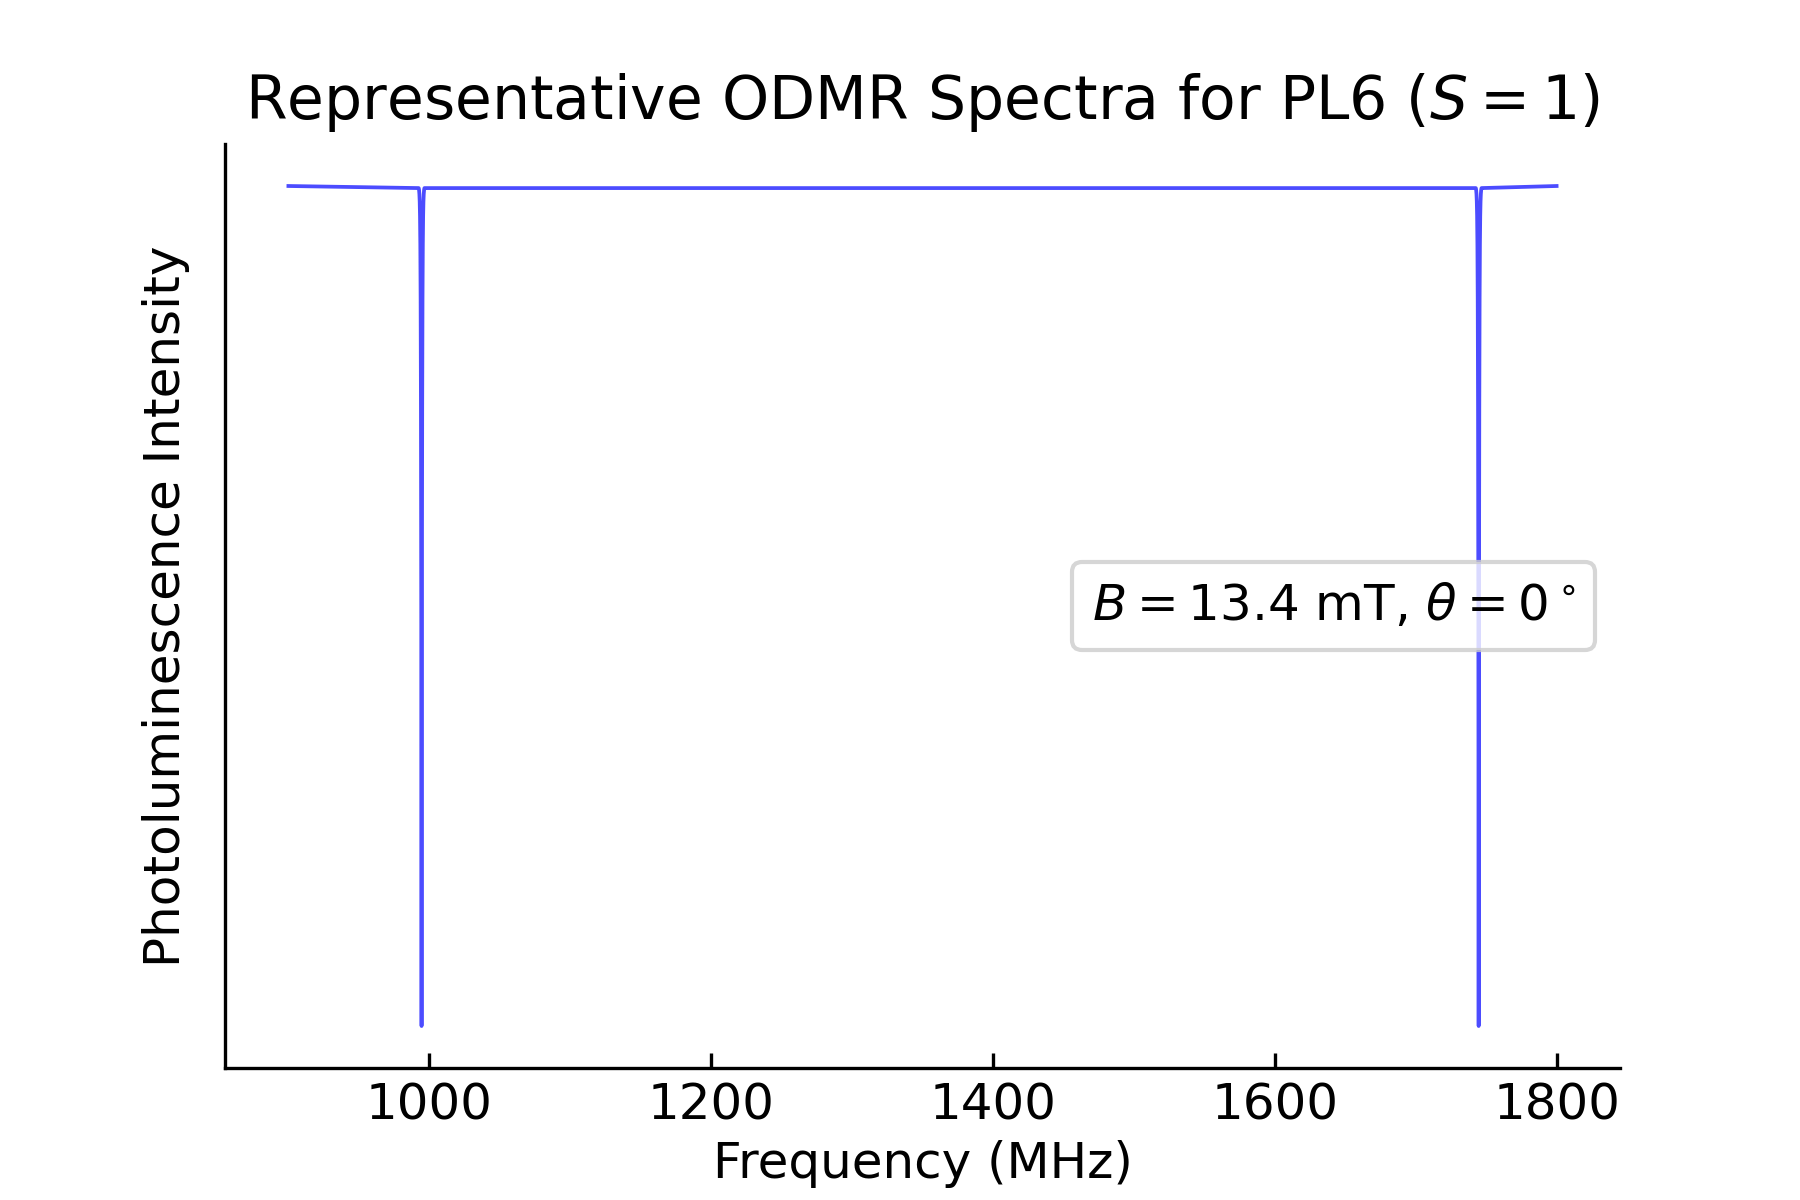
\includegraphics[width=\textwidth]{figures/PL6ODMRSpectra_theta_0_to_90.png}
	\end{center}
	\caption{ODMR/Energy level plot showing the reduction of the effective parallel $\vec{B}$ field with increasing $\theta$.}
	\label{fig:}
\end{figure}


\subsection{$S=1$ Vector Magnetometry}
Vector magnetometry with a $S=1$ system can be achieved by comparing the relative intensities from defects known to be at specific angles.

For example, in diamond the nitrogen vacancy is aligned with the tetragonal crystal structure and thus may take one of four orientations as illustrated in Figure \ref{fig:dnv_orientations}.

\begin{figure}[h]
	\begin{center}
		% \missingfigure{Sketch of DNV and possible defect orientations.}
		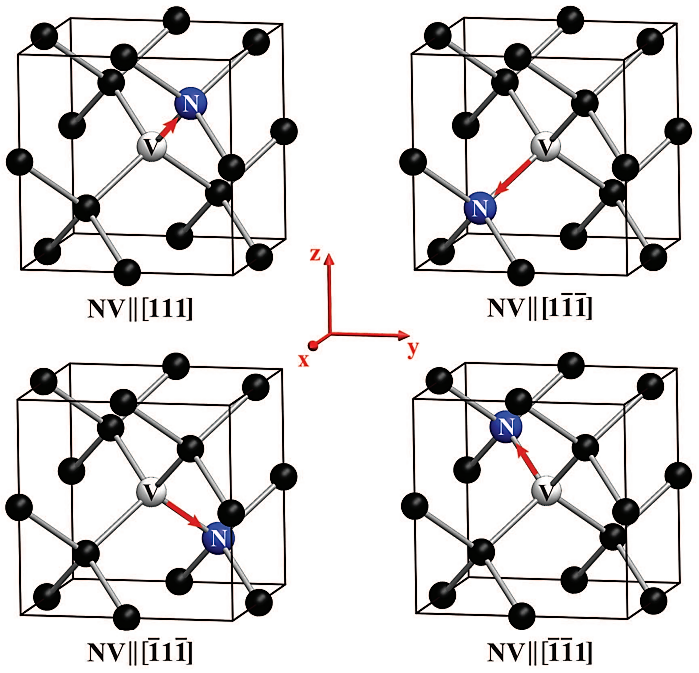
\includegraphics[width=0.45\textwidth]{figures/four_possible_NV_orientations.png}
	\end{center}
	\caption{Diagram showing the four possible orientations of NV centers in diamond \cite{pham}.}\label{fig:dnv_orientations}
\end{figure}


The 4 possible DNV orientations in the lattice are $111$, $1\overline{11}$, $\overline{1}1\overline{1}$ and $\overline{11}1$.
Once the projections of the magnetic field along these axes have been measures, we reconstruct the magnetic field in the laboratory frame.

The ODMR sprectrum for a sample of diamond with approximately equal distribution of the four defect orientations.

% # file:///home/conner/Downloads/e2015-60080-1.pdf
\td{Finish typing - link in comments}
The measured field components $m_i$ do not directly give the magnetic field $B_i$, but are affected by some noise in-
herent to the measurement which is accounted for using a maximum-likelihood method.

% The direction of $\vec{B}$ relative to the crystal lattice can then be determined by solving 
% \begin{equation}
%     \underbrace{
%     \frac{1}{\sqrt{3}}
%     \begin{pmatrix}        
%         1 & 1 & 1 \\ 
%         -1 & -1 & 1 \\ 
%         -1 & 1 & -1 \\ 
%         1 & -1 & -1 
% \end{pmatrix}}_{N}
%     \mathbf{\hat{B}} = 
%     \underbrace{
%     \begin{pmatrix}
%         \cos\theta_1 \\
%         \cos\theta_2 \\
%         \cos\theta_3 \\
%         \cos\theta_4 \\
%     \end{pmatrix}
% }_{\mathbf{c}}
%     \label{eq:}
% \end{equation}
% For which a solution may be determined 
% \begin{equation}
%     \mathbf{\hat{B}} = \left(N^T N\right)^{-1} N^T \mathbf{c}.   
%     \label{eq:}
% \end{equation}
%
% With knowledge of .. \td{Need to finish writing about knowing the miller index family of crystal can convert miller vector to lab vector}. 
%

\cite{Balasubramanian2008}
\td{Need to also look at this method and type up}

% \begin{tcolorbox}[colback=ediblue!5!white,colframe=ediblue!75!black,title={$S=1$ Magnetometry Summary}]
% \end{tcolorbox}

% \begin{summary}{%
% 		\subsection{$S=1$ Magnetometry Summary}%
% 		\label{spin1_magnetometry}%
%         \vspace{-0.5em}
% 	}%
%
% 	We may achieve vector magnetometry using a triplet state if
% \end{summary}

\begin{summary}{$S=1$ Magnetometry Summary}{sum:spin1magnet}

	We may achieve vector magnetometry using a triplet state if
	\begin{enumerate}
		\item We can identify three lines.
		\item We can use this equation which we have already written and we link:
		      \begin{equation}
                  \tcbhighmath{B_0 = \frac{f_1 - f_2}{2 \gamma}}
			      \tag{\ref{eq:s1_parallel_magnetometry}}
		      \end{equation}
	\end{enumerate}


\end{summary}

\section{$S=1$ Magnetometry}\label{s1_magnetometry}
We will consider the use of a SiC divacancy e.g. PL5 or PL6.

We begin with our total Hamiltonian \eqref{eq:total_hamiltonian}. We will consider the system under the influence of only the $\vec{B}$ field, so can remove the Stark effect terms. Additionally, for $S=1$ we may reduce the constant terms \cite{Christle2014} leaving
\begin{equation}
	H = g\mu_b \hat{\vec{S}}\cdot\vec{B} + D\hat{S}_z^2 + E (\hat{S}_x^2 - \hat{S}_y^2).
	\label{eq:s1_magnetometry_hamiltonian}
\end{equation}

By transforming into spherical coordinates, with $\theta, \phi$ the azimuthal and polar angle respectively and $B = |\vec{B}|$
\begin{equation}
	\begin{align}
		B_x & = & g\mu_b B \cos\varphi \sin\theta \\
		B_y & = & g\mu_b B \sin\varphi \sin\theta \\
		B_z & = & g\mu_b B \cos\theta
	\end{align}
	\label{eq:polar_transform}
\end{equation}
then substituting the spin operators \eqref{eq:s1_spin_operators} we find
\begin{equation}
	H = \begin{pmatrix}
		D + g\mu_b B \cdot \cos \theta                                       & \frac{g\mu_b B}{\sqrt{2}} \cdot e^{-i\cdot \varphi} \cdot \sin\theta & E                                                              \\
		\frac{g\mu_b B}{\sqrt{2}} \cdot e^{i \cdot \varphi} \cdot \sin\theta & 0                                                                    & \frac{g\mu_b B}{\sqrt{2}} e^{-i\cdot \varphi} \cdot \sin\theta \\
		E                                                                    & \frac{g\mu_b B}{\sqrt{2}} \cdot e^{i \cdot \varphi} \cdot \sin\theta & D - g\mu_b B \cdot \cos \theta
	\end{pmatrix}.
	\label{eq:s1_magnetometry_hamil_spherical_matrix}
\end{equation}



\subsection{$\vec{B}$ Parallel to Defect}
It is straightforward to show from \eqref{eq:s1_magnetometry_hamil_spherical_matrix} that if the magnetic field is applied parallel to the defect axis ($\theta = 0$) then the matrix reduces to
\begin{equation}
	H_{} = \begin{pmatrix}
		D + g\mu_b B & 0 & E          \\
		0            & 0 & 0          \\
		E            & 0 & D-g\mu_b B
	\end{pmatrix},
	\label{eq:reduced_H_s1_magnetometry_matrix}
\end{equation}
with eigenvalues

\begin{equation}
	E_x = E_y = D \pm \sqrt{(g\mu_b B)^2  + E^2}, \; E_z = 0.
	\label{eq:reduced_H_NV_eigenvalues}
\end{equation}

The uniaxial symmetry of the SiC divacancy means $D \ll E$. Further, we expect to sense in the range where $g\mu_b B \gg D$ therefore we may write the eigenvalues as
\begin{equation}
	E_x = E_y \simeq D \pm g\mu_b B, \; E_z = 0.
	\label{eq:reduced_H_NV_eigenvalues}
\end{equation}

    That is, for the transitions between $m_s=0$ and $m_s = \pm 1$\footnote{These are the allowed transitions for optical depopulation due to selection rules. This may be simply thought of as a helicity conservation as the photon is a $S=1$ particle.}, the difference is energy reflected in the EPR spectra (visualised in figure \ref{fig:linear_zeeman} (right)) is the Zeeman energy
\begin{equation}
	\Delta E = 2g \mu_B B =  2\gamma B.
	\tag{\ref{eq:zeeman_energy}}
\end{equation}
\begin{figure}[H]
    \begin{center}
        % 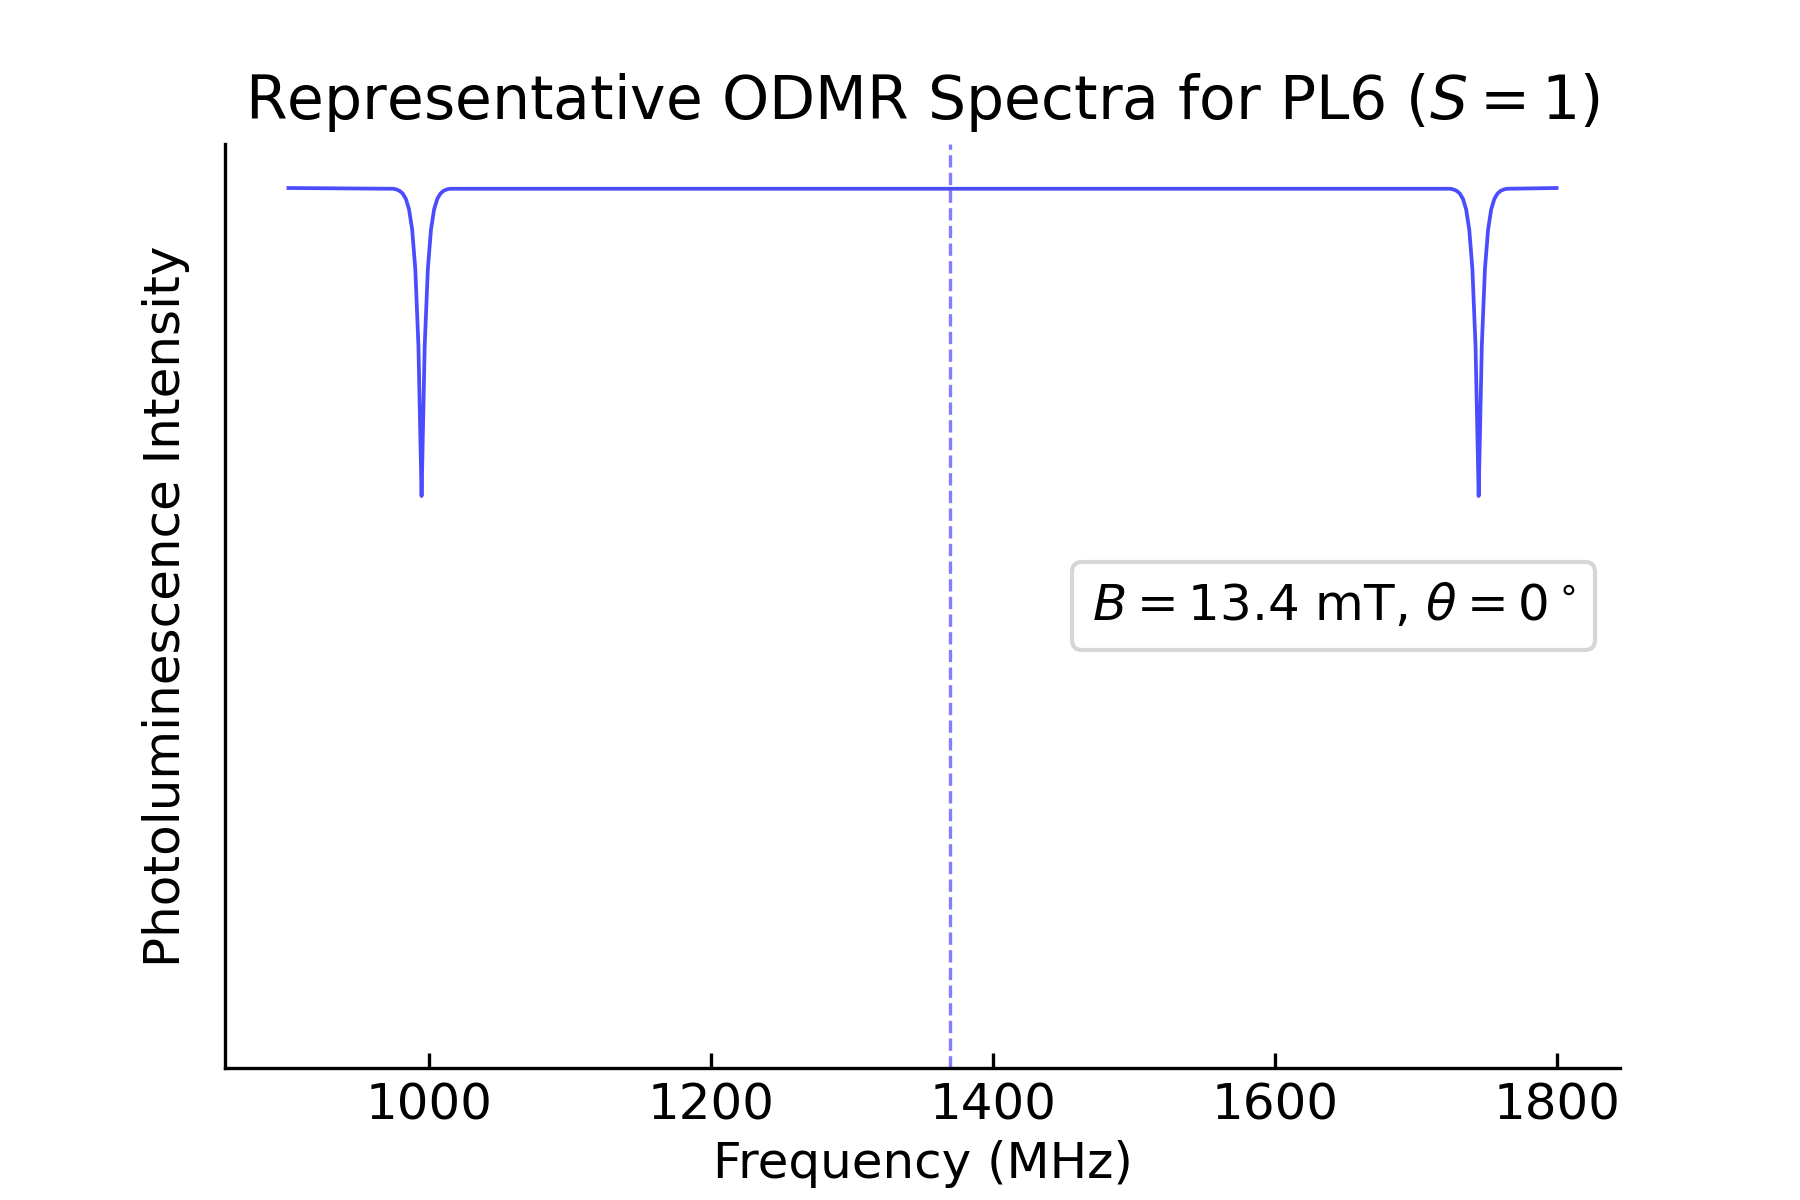
\includegraphics[width=0.49\textwidth]{figures/ODMR-s1magnet-1.png}
        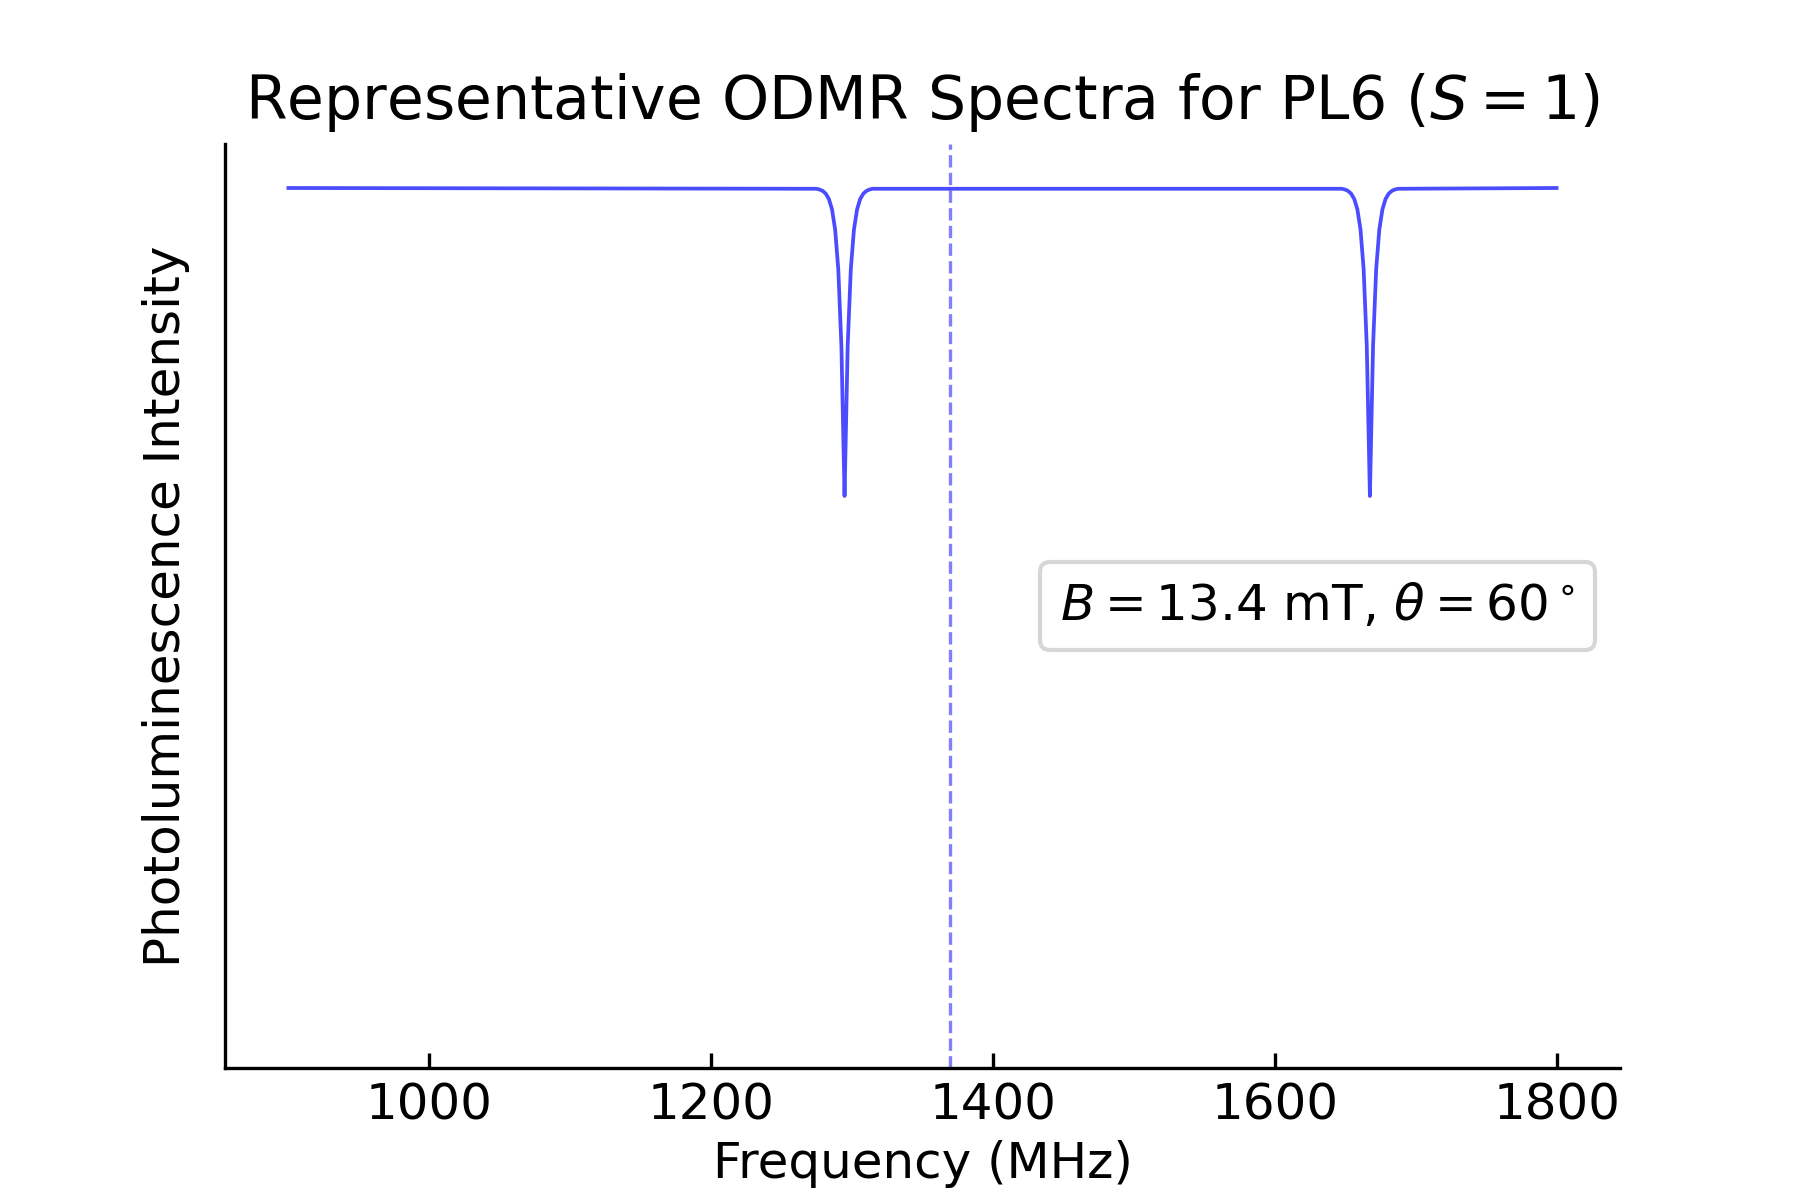
\includegraphics[width=0.49\textwidth]{figures/ODMR-s1magnet-2.png}
        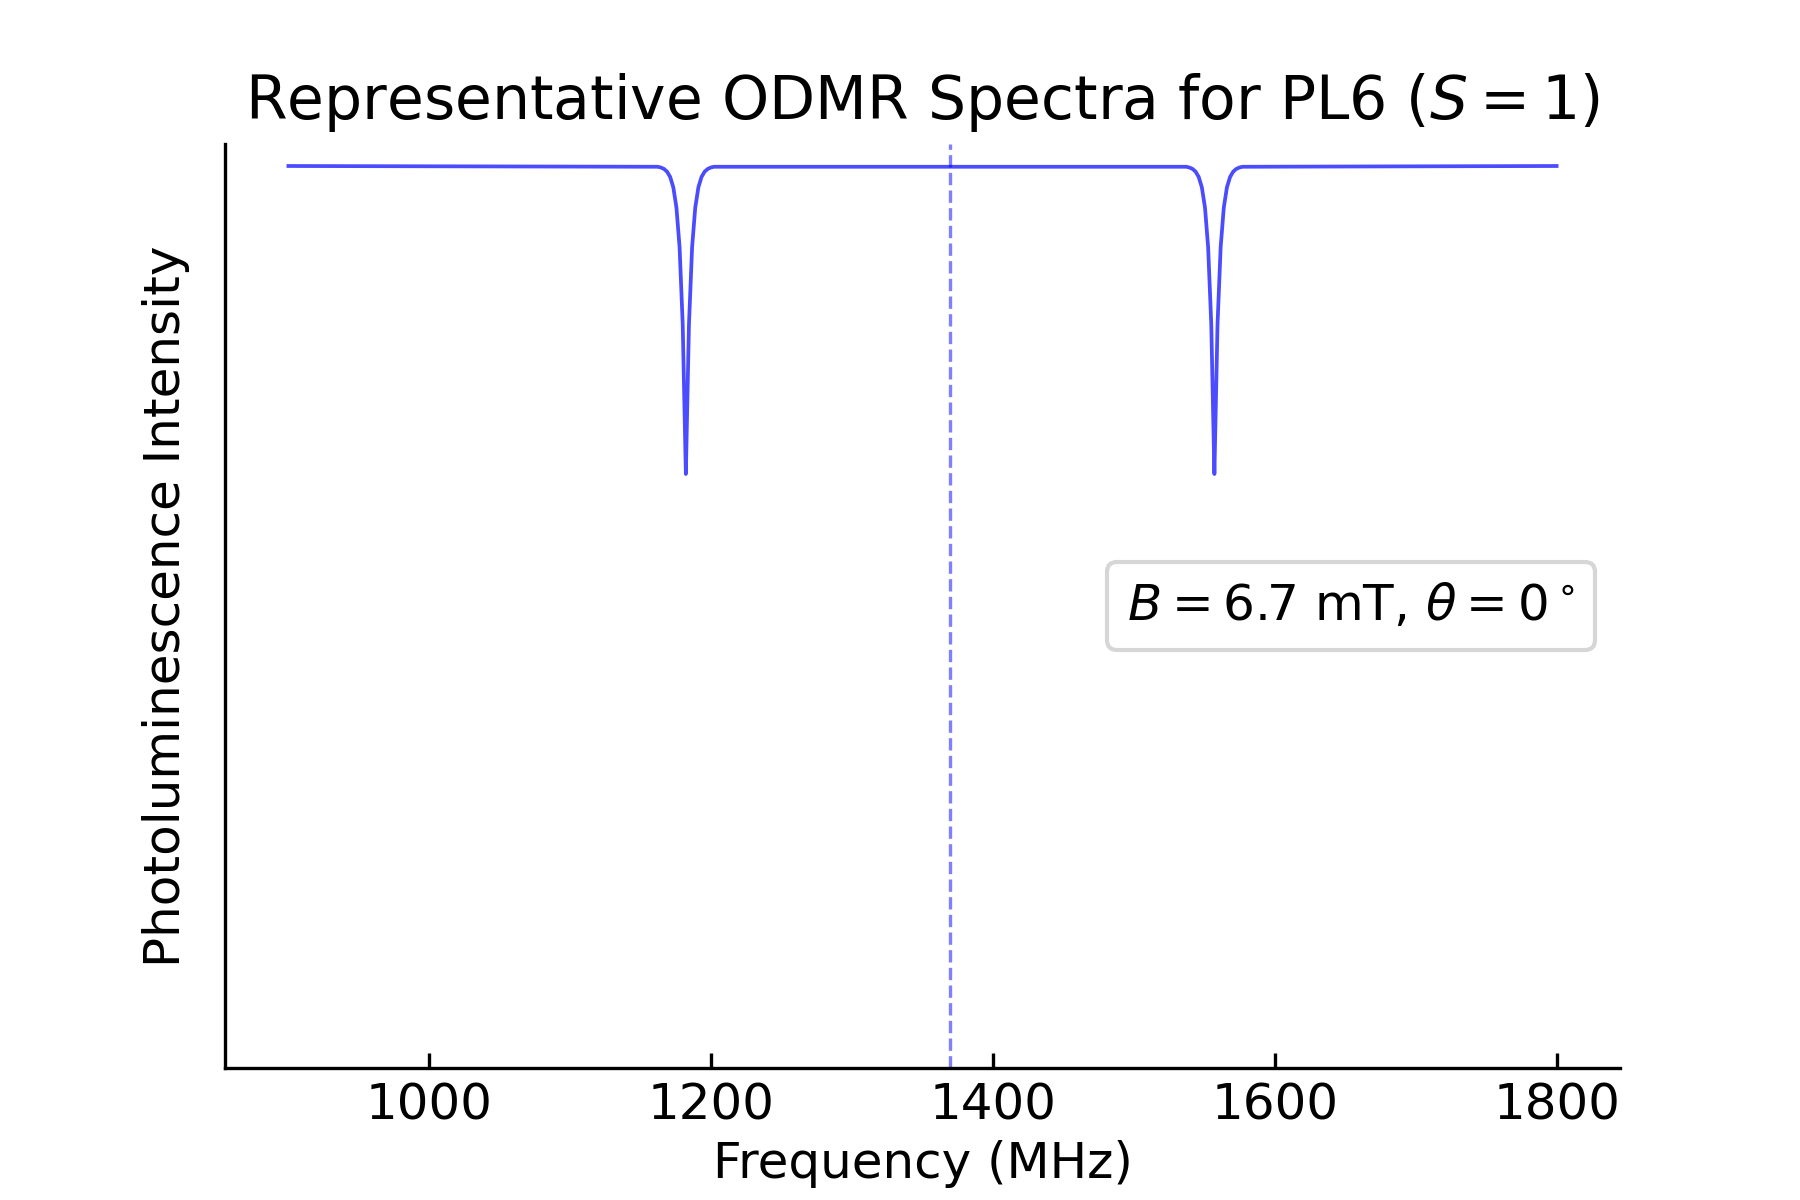
\includegraphics[width=0.49\textwidth]{figures/ODMR-s1magnet-3.png}

    \end{center}
    \caption{Representative PL6 ODMR spectra showing linear dependence of frequency difference on $B\cos\theta$ and the ZFS shifting of the spectra when $\theta > 0$. Dashed vertical line indicates $D$.}\label{fig:linear_zeeman}
\end{figure}
Thus, for CW-ODMR the difference between the two frequencies $f_1 > f_2$ is directly proportional to $B$
\begin{equation}
	f_1 = D + \gamma B,  \quad f_2 = D - \gamma B
	\label{eq:}
\end{equation}

It is then straightforward to calculate $B$ using
\begin{equation}
	B = \frac{f_1 - f_2}{2 \gamma}.
	\label{eq:s1_parallel_magnetometry}
\end{equation}


\subsection{Vector Magnetometry}
By returning to \eqref{eq:s1_magnetometry_hamil_spherical_matrix} it immediately follows from the characteristic equation that eigenvalues $\lambda$ satisfy
\begin{equation}
	0 = \lambda^3 - 2\lambda^2 D + \frac{D (g\mu_b B)^2}{2} + \lambda(D^2 - E^2 - (g\mu_b B)^2) - \frac{1}{2}(g\mu_b B)^2\underbrace{\left(D \cos(2\theta) - 2  E \cos(2\varphi)  \sin^2(\theta)\right)}_{\eta}
	\label{eq:nv_spherical_characteristic_equation}
\end{equation}
where $\eta$ depends only on the ZFS parameters and the vector of the applied $\vec{B}$ field.

This allows a more general determination of $B$ from the ODMR spectra using
\begin{equation}
	B = \frac{\sqrt{\frac{1}{3} \left(f_1^2 - f_1 f_2 + f_2^2 -D^2 -3E^2\right)}}{g \mu_B}.
	\label{eq:spin1_magnet_magnitude}
\end{equation}

Further we may find $\eta$ using
\begin{equation}
	\eta = \frac{-7 D^3 - 4f_1^3 + 6 f_1^2 f_2 + 6f_1 f_2^2 - 4f_2^3 + 3D(9E^2 + f_1^2 -f_1 f_2 + f_2^2)}{9(D^2 + 3E^2 - f_1^2 + f_1f_2 - f_2^2)}.
	\label{eq:}
\end{equation}
Again, exploiting the uniaxial symmetry of our systems we may reduce our expression for $\eta$
\begin{equation}
	\eta = D \cos(2\theta) - 2  E \cos(2\varphi) \sin^2(\theta) \simeq D \cos2\theta
	\label{eq:}
\end{equation}
therefore with just two frequencies and knowledge of the ZFS parameters, whilst a complete vector cannot be reconstructed, we may determine the magnitude and azimuthal angle of an applied $\vec{B}$ field
\begin{equation}
	\theta = \frac{\cos^{-1} (\eta/D)}{2}
	\label{eq:spin1_magnet_theta}
\end{equation}


\begin{summary}{$S=1$ Magnetometry Summary}{sum:spin1magnet}
	We may achieve angle resolved magnetometry using a $S=1$ system provided:
	\begin{enumerate}
        \item We can resolve \textbf{two frequencies} corresponding to the defect in the CW-ODMR spectra.
		% \item We know the ZFS parameters $D$ and $E$.
		\item The ZFS parameters $D$ and $E$ are well known.
		\item We can determine the magnitude using
		      \begin{equation}
			      \tcbhighmath{B = \frac{\sqrt{\frac{1}{3} \left(f_1^2 - f_1 f_2 + f_2^2 -D^2 -3E^2\right)}}{g \mu_B}.}
			      \tag{\ref{eq:spin1_magnet_magnitude}}
			      % \tcbhighmath{g\mu_b B = \frac{f_1 - f_2}{2 \gamma}}
			      % \tag{\ref{eq:s1_parallel_magnetometry}}
		      \end{equation}
		\item We can determine the azimuthal angle using
		      \begin{equation}
			      \tcbhighmath{
				      \theta = \frac{\cos^{-1} (\eta/D)}{2}.
			      }
			      \tag{\ref{eq:spin1_magnet_theta}}
		      \end{equation}
	\end{enumerate}
\end{summary}

\section{$S = 3/2$ Magnetometry}
Now we will consider the use of a SiC Silicon vacancy, specifically V2.
For a general $S=3/2$ system we begin with \eqref{eq:total_hamiltonian}.
% The V2 defect has ZFS parameter $E=0$ \cite{Nagy2019} thus we may remove that term. 
Again we will only consider the influence of the $\vec{B}$ field leaving
\begin{equation}
	H = g\mu_b \hat{\vec{S}}\cdot\vec{B} + D\left(\hat{S}_z^2 - \frac{1}{3}S(S+1)\right) + E(\hat{S}_x^2 - \hat{S}_y^2).
	\label{eq:s1.5_magnetometry_hamiltonian}
\end{equation}

% V2 
\cite{PhysRevApplied.4.014009}
\cite{PhysRevB.92.115201}
\cite{1505.06914}
\todo[inline]{Distribute refs}

If the ZFS interaction of the $S=3/2$ defect is sufficiently strong, the eigenvalues of the
spin Hamiltonian show a strong dependence on the orientation of the applied magnetic field.

This induces a non-linear shift of resonance transitions in EPR frequencies, which is seen in the ODMR spectra. Like $S=1$, this allows information about the applied external magnetic field to be extracted from EPR spectra provided the ZFS parameters are known.

In zero magnetic field the $V_{\ce{Si}}$ V2 vacancy has an ODMR line maximum ($D$) around 70 MHz with very weak dependence on temperature.
% That is, the ZFS parameter is known and resistant to the environmental influence of temperature. 

% In a $S=3/2$ spin system the orientation related terms are, like for $S=1$ systems, in the eigenvalue equation. 
% This results in the orientation dependent shift of EPR frequencies which are not explained by $g \mu_B B_0$ as they are for $S=1$. 

% Therefore in order to 
In order to
reconstruct the energy eigenstates we must use the observed resonant energies. There are $2S +1 $ states for a system with spin $S$ from which $2S$ transition frequencies may be found. Therefore, we may find up to three EPR frequencies.


% Applying a magnetic field $B_0$ along the defect axis, $\theta = 0$, 

% As stated, the V2 $V_{\ce{Si}}$ has $E=0$ so trivially $E \ll D$ and a uniaxial symmetry exists therefore the Hamiltonian for the system is given as in equation \ref{}\td{ref correct hamiltonian}. Here we use the 4-dimensional $S=3/2$ matrix representation 
% \begin{equation}
%     \label{eq:}
% \end{equation}
%     \td{Add spin 3/2 matrices} 
%
%     For this defect, 

Using the same polar co-ordinate conversion as \eqref{eq:polar_transform} and $B = |\vec{B}|$ we may write the Hamiltionian in matrix form as
\begin{equation}
	\begin{align}
		H & = \\
		  &
		\resizebox{\hsize}{!}{%
			\begin{pmatrix}
				D + \frac{3}{2} g \mu_B B \cdot  \cos\theta                                  & \frac{\sqrt{3}}{2} g \mu_B B \cdot \sin\theta \cdot e^{-i\varphi} + \sqrt{3} E & 0                                                                            & 0                                                                             \\
				\frac{\sqrt{3}}{2} g \mu_B B \cdot \sin\theta \cdot e^{i\varphi} + \sqrt{3}E & \frac{1}{2}g \mu_B B \cos \theta-D                                             & g \mu_B B \cdot \sin\theta \cdot \cos\varphi + 2E                            & 0                                                                             \\
				0                                                                            & g \mu_B B \cdot \sin\theta \cdot \cos\varphi + 2E                              & -\frac{1}{2}g\mu_B B \cdot \cos\theta - D                                    & \frac{\sqrt{3}}{2} g \mu_B B \cdot \sin\theta \cdot e^{-i\varphi} + \sqrt{3}E \\
				0                                                                            & 0                                                                              & \frac{\sqrt{3}}{2} g \mu_B B \cdot \sin\theta \cdot e^{i\varphi} + \sqrt{3}E & D - \frac{3}{2} g \mu_B B \cdot  \cos\theta
			\end{pmatrix}.%
		}
	\end{align}
	\label{eq:s1.5_magnetometry_hamil_spherical_matrix}
\end{equation}


\subsection{$\vec{B}$ Parallel to Defect}
Considering $B$ parallel to the defect axis and  we find \cite{Kirmse1995} the Hamiltonian reduces to
\begin{equation}
	H = \begin{pmatrix}
		D + \frac{3}{2} g \mu_B B & \sqrt{3}E               & 0                        & 0                               \\
		\sqrt{3}E                 & \frac{1}{2}g \mu_B B -D & 2E                       & 0                               \\
		0                         & 2E                      & -\frac{1}{2}g\mu_B B - D & \sqrt{3}E                       \\
		0                         & 0                       & \sqrt{3}E                & D - \frac{3}{2} g \mu_B B \cdot
	\end{pmatrix}%
	\label{eq:}
\end{equation}
with eigenvalue equations given by
\begin{equation}
	\lambda = \frac{1}{2}g\mu_B B \pm \sqrt{(D + g\mu_B B)^2 + 3E^2}
	\text{ or, }
	\lambda = -\frac{1}{2} g\mu_B B \pm \sqrt{(D-g\mu_B B)^2 + 3E^2}.
	% \label{eq:}
\end{equation}
Which we further simplify for the Silicon vacancy as $E=0$ \cite{Nagy2019} to
\begin{equation}
	H = \begin{pmatrix}
		D + \frac{3}{2} g \mu_B B & 0                       & 0                        & 0                         \\
		0                         & \frac{1}{2}g \mu_B B -D & 0                        & 0                         \\
		0                         & 0                       & -\frac{1}{2}g\mu_B B - D & 0                         \\
		0                         & 0                       & 0                        & D - \frac{3}{2} g \mu_B B
	\end{pmatrix}%
	\label{eq:}
\end{equation}

% \begin{equation}
% 	\lambda = \frac{1}{2}g\mu_B B \pm (D + g\mu_B B)
% 	\text{ or, }
% 	\lambda = -\frac{1}{2} g\mu_B B \pm (D-g\mu_B B).
% 	% \label{eq:}
% \end{equation}
which is diagonal so we may immediately read off
\begin{equation}
	\begin{align}
		\lambda_1 & =   & 3/2   g \mu_B B & +  D  \\
		\lambda_2 & =   & 1/2   g \mu_B B & -D    \\
		\lambda_3 & = - & 1/2  g \mu_B B  & -D    \\
		\lambda_4 & = - & 3/2  g \mu_B B  & +  D.
	\end{align}
	\label{eq:}
\end{equation}

\todo[inline]{a sentence to wrap this up}


\subsection{Vector Magnetometry}
Coming back to \eqref{eq:s1.5_magnetometry_hamil_spherical_matrix} we find the eigenvalue equation for a general $S=3/2$ system to be
\begin{equation}
	\begin{align}
		 & \lambda^4 - \left(2D^2 + 6E^2  + \frac{5}{2}(g\mu_B B_0)^2 \right)\lambda^2 - 2 (g \mu_B B_0)^2 \left(D(3 \cos^2 \theta -1) + 3E \sin^2\theta \cos 2\varphi \right)\lambda \\
		 & +\frac{9}{16}(g \mu_B B_0)^4 + D^4 - \frac{1}{2}D^2 (g \mu_B B_0)^2 - D^2 (g \mu_B B_0)^2 (3 \cos^2 \theta - 1) + 3E^2(3E^2 + 2D^2)                                        \\
		 & + E(g\mu_BB_0)^2 (6D \sin^2\theta \cos 2\varphi + \frac{9}{2}E \cos2\theta) = 0.
	\end{align}
	\label{eq:V2_eigenvalue_equation}
\end{equation}

We may write the general equation for the eigenvalues as
\begin{equation}
	\sum_{n=0}^{2S+1} C_n \lambda^n = 0
	\label{eq:}
\end{equation}
we then substitute each eigenvalue $\lambda_i$ into this general expression to obtain $2S + 1$ equations.

The goal is now to remove all $\lambda_i$ terms by considering instead the transition frequencies between eigenstates, which are observed in the ODMR spectra. The energy states are not in general sorted with respect to the energy values, so we use the convention that $\lambda_i > \lambda_{i-1}$.

To reduce our number of equations to $2S-1$ we make the substitutions
$$\lambda_i + \underbrace{\lambda_{i+1} - \lambda_{i}}_{f_{i+1, i}} = \lambda_{i+1},
	\qquad\lambda_i - \underbrace{(\lambda_{i} - \lambda_{i-1})}_{f_{i, i-1}} = \lambda_{i-1}$$
for each $i = 2, \dots, 2S$ and calculate both
$$\sum_{n=0}^{2S +1} \frac{C_n \left((\lambda_i + f_{i+1, i})^n - \lambda_i^n\right)}{C_{2S+1}} = 0\text{ and } \sum_{n=0}^{2S +1}\frac{C_n \left((\lambda_i - f_{i, i-1})^n - \lambda_i^n\right)}{C_{2S + 1}} = 0$$
to find two new simultaneous equations
$$\sum_{n=0}^{2S} C_{i,n}' \lambda_i^n = 0 \text{ and } \sum_{n=0}^{2S} C''_{i,n}\lambda_i^n = 0.$$

We may combine these as
$$\sum_{n=0}^{2S} \frac{C'_{i,n}\lambda_i^n}{C'_{i,2S}}-\frac{C''_{i,n} \lambda_i^n}{C''_{i, 2S}} = 0$$
to obtain an equation for the eigenvalue of the energy eigenstate $\ket{i}$ where $i = 2, \dots, 2S$:

\begin{equation}
	\sum_{n=0}^{2S -1} C_{i,n}^{(2S-1)} \lambda_i^n = 0.
	\label{eq:refmenowpls}
\end{equation}

This process is repeated until only one linear equation exists for each eigenvalue, which may be expressed in terms of resonant energies. $f_{i, i-1}$ can then be substituted to find expressions for all other eigenvalues.
% For 
% the V2 $V_{\ce{Si}}$, 
% we 
We
obtain equations for $\lambda_2$ expressed in terms of $f_{2,1}, f_{3,2}$ and $\lambda_3$ expressed in terms of $f_{3,2}, f_{4,3}$.

Finally, using $f_{3,2} = \lambda_3 - \lambda_2$ we find formulas for each eigenvalues in terms of the resonant frequencies:

\begin{eqnarray}
	\lambda_1 = -\frac{3}{4}f_{2,1} - \frac{1}{2} f_{3,2} - \frac{1}{4} f_{4,3}\\
	\lambda_2 = \frac{1}{4}f_{2,1} - \frac{1}{2}f_{3,2} - \frac{1}{4} f_{4,3} \\
	\lambda_3 = \frac{1}{4}f_{2,1} + \frac{1}{2}f_{3,2} - \frac{1}{4} f_{4,3} \\
	\lambda_4 = \frac{1}{4}f_{2,1} + \frac{1}{2}f_{3,2} + \frac{1}{4} f_{4,3}.
\end{eqnarray}

We substitute one of these expressions into one of the equations of the form of equation \eqref{eq:refmenowpls} and we obtain
\begin{equation}
	\begin{align}
		5(g\mu_B B)^2 & =\left(\frac{\sqrt{3}}{2}f_{4,3} + f_{3,2}  + \frac{\sqrt{3}}{2}f_{2,1}\right)^2 \\
		              & +(1 - \sqrt{3}) (f_{4,3} + f_{2,1})f_{3,2} - f_{4,3}f_{2,1} - 4(D^2 + 3E^2).
	\end{align}
	\label{eq:V2_magnitude}
\end{equation}

We also find a $S=3/2$ $\eta$ which is again useful for angle resolution as it is dependent on the ZFS parameters, $\theta$ and $\varphi$

\begin{equation}
	\eta \equiv E(2\cos^2\varphi \sin^2 \theta + \cos^2\theta) + D\cos^2 \theta
	\label{eq:eta}
\end{equation}

which in terms of the resonant frequencies is given by
\begin{equation}
	\begin{align}
		 & \eta =                                                                                                                                                              \\
		 & \frac{4\left(8(D + 3E) + 5(f_{4,3}-f_{2,1})\right)(g\mu_B B)^2 + (f_{4,3} - f_{2,1})\left(16(D^2 + 3E^2) - (f_{4,3}-f_{2,1})^2 - 4f_{3,2}^2\right)}{96(g\mu_B B)^2}
	\end{align}
	\label{eq:eta_resonant}
\end{equation}
where $(g \mu_B B)^2$ may be determined in terms of the frequencies as \eqref{eq:V2_magnitude}.


Overall, this shows that if the ZFS is known and three EPR frequencies are observed, the applied magnetic field strength can be found using \eqref{eq:V2_magnitude}.


% \subsection{$\vec{B}$ Parallel to Defect Axis}

% The simplest possible cashen $\theta = 0$ there is no super-position of states and selection rules dictate that the only transitions available 



% For $B_0$ perpendicular to the defect axis we find:
% \begin{equation}
% 	\begin{align}
% 		        & \lambda = \frac{1}{2}g\mu_B B_0 \pm \sqrt{(g\mu_B B_0)^2 + D^2  + 3E^2 - (D - 3E)g\mu_B B_0}\text{ or, } \\
% 		\lambda & = -\frac{1}{2}g\mu_B B_0 \pm \sqrt{(g\mu_B B_0)^2 + D^2 + 3E^2 + (D-3E)g\mu_B B_0}.
% 	\end{align}
% \end{equation}
%


Since $E = 0$, $E \ll D$ for the Silicon vacacny, we may approximate $\eta$ defined in equation \eqref{eq:eta} to
\begin{equation}
	\eta \simeq D \cos^2 \theta.
	\label{eq:}
\end{equation}

By exploiting this approximation, we can determine the azimuthal angle that the magnetic field vector makes with the defect axis, however at this stage we may not determine anything about the $x,y$ components of the vector.

To do so we explicitly compute $\eta$ using equation \eqref{eq:eta_resonant} then we find the azimuthal angle as
\begin{equation}
	\theta = \cos^{-1}\sqrt{\frac{\eta}{D}}
	\label{eq:vector_theta}
\end{equation}


% \subsection{$S = 3/2$ Vector Magnetometry}
% Vector magnetometry is achieved in the case of the DNV as described in section \ref{dnv_vector} \td{link reference} and theoretically a similar approach is possible in SiC. There exists two distinct and differently oriented Silicon vacancies in 4H-SiC and three in 6H-SiC \cite{Janzn2009}. In practice however, in practice at least one of the defects in each polytope is difficult to observe at room temperature making this approach unsuitable for vector magnetometry.
%
In a general $S = 3/2$ system, ambiguity is found when computing $\theta$ using equation \eqref{eq:vector_theta} as the EPR frequencies can not be mapped to specific transitions.

\todo[inline]{Finish spin 3/2 magnetometry section, reference using ref B fields and discuss method in paper}.

{\color{edired}
The following approach exploits the fact that a crossing of resonant frequencies occurs at a given angle (see figure \ref{fig:resonant_crossing_V2}). The method should be considered for $g\mu_B B_0 \gg 2\sqrt{D^2 + 3E^2}$ explicitly as interactions such as level anti-crossing produce a complex spectra \cite{Degen2008} when $g\mu_B B_0 \approx 2\sqrt{D^2 + 3E^2}$ and the invariance of a particular EPR frequency when $g \mu_B B_0 \ll 2 \sqrt{D^2 + 3E^2}$ makes determination of the polar angle $\theta$ impossible.

\begin{figure}[H]
	\begin{center}
		% \includegraphics[width=0.95\textwidth]{figures/}
		\missingfigure{Plot showing the crossing of EPR frequencies at high field and low field in Spin 3/2 system as theta varies}
	\end{center}
	\caption{\td{write caption}}\label{fig:resonant_crossing_V2}
\end{figure}

% \begin{group}
% 	\color{gray}
% 	At a high B0 field (gμB B0  ZFS),
% 	B0 can be obtained from the observed ESR spectra but
% 	the polar angle cannot be determined due to the ambigu-
% 	ity of differentiating two outer transitions. In contrast,
% 	at low gμB B0 ( ZFS), as long as one can explicitly
% 	identify at least three transitions including the allowed
% 	lowest energy transition, the external magnetic field vec-
% 	tor can be reconstructed. In the field strength compara-
% 	ble to the ZFS, it is hard to find a useful scheme because
% 	very complex patterns appear due to mixing of some of
% 	the eigenstates. In the case of the NV centers in dia-
% 	mond (ZFS/h=2.87 GHz), this missing range is around
% 	∼ 100 mT . The VSi in SiC can fill out this gap since its
% 	ZFS is quite small (ZFS/h ∼ 100 MHz) thus this mag-
% 	netic field range can be considered as a high field range
% 	in which the three necessary transitions are well observ-
% 	able25,29, and at least the field strength can be experi-
% 	mentally determined. When the VSi in SiC is used to
% 	realize such schemes at sub-mT, if the lowest transition
% 	energy is observable by ELDOR, one can determine both
% 	B0 and θ without ambiguity.
% 	% Even if ELDOR is not avail-
% 	% able, thanks to the additional transitions that appear at
% 	% low fields, the field strength can be determined.
% 	% The magic angle terms in the eigenvalue equation al-
% 	% low for an alternative method to use S=3/2 systems as
% 	% a DC vector magnetometer. If the S=3/2 spins fixed
% 	% in a crystal can be rotated around the rotational axis,
% 	% the unambiguous determination of the applied magnetic
% 	% field vector is feasible by monitoring the linewidth of the
% 	% observed ESR spectra while the symmetry axis of the
% 	% crystal is oriented at θm relative to the rotational axis
% 	% and the rotational axis is moving. This configuration
% 	% also can be realized by producing an array of the crystals
% 	% such that the symmetry axes of each crystal form a cone
% 	% whose opening angle is twice the magic angle.
% 	% These findings provide a better understanding of the
% 	% S=3/2 electronic spin Hamiltonian, especially at low
% 	% fields. They also provide an outlook for the application of
% 	% VSi in SiC to quantum magnetometry which is promising
% 	% thanks to the electrical properties of SiC, which outstand
% 	% the host material of the NV centers, and the mature fab-
% 	% rication technology, which allows an efficient fabrication
% 	% of electronic devices even at the atomic scale48
% \end{group}


% In addition, it is demonstrated that the observation of the central line of the TV2a center of S = 3/2 has been achieved by pulsed-ELDOR
\cite{Isoya2008}


% \cite{Kraus2014}


}

\begin{summary}{$S=3/2$ Magnetometry Summary}{sum:spin1.5magnet}
	We may achieve angle resolved magnetometry using a $S=3/2$ system provided:
	\begin{enumerate}
		\item We can resolve \textbf{three frequencies} corresponding to the defect in the CW-ODMR spectra.
              \todo[inline]{add the specific freq we need.}
		\item We know the ZFS parameters $D$ and $E$.
		\item We can determine the magnitude using
		      \begin{equation}
			      \tcbhighmath{
				      \begin{align}
					      5(g\mu_B B)^2 & =\left(\frac{\sqrt{3}}{2}f_{4,3} + f_{3,2}  + \frac{\sqrt{3}}{2}f_{2,1}\right)^2 \\
					                    & +(1 - \sqrt{3}) (f_{4,3} + f_{2,1})f_{3,2} - f_{4,3}f_{2,1} - 4(D^2 + 3E^2).
				      \end{align}
			      }
			      \tag{\ref{eq:V2_magnitude}}
			      % \tcbhighmath{g\mu_b B = \frac{f_1 - f_2}{2 \gamma}}
			      % \tag{\ref{eq:s1_parallel_magnetometry}}
		      \end{equation}
              including the 
		\item We can determine the azimuthal angle using
		      \begin{equation}
			      \tcbhighmath{
				      \theta = \cos^{-1}\sqrt{\frac{\eta}{D}}
			      }
			      \tag{\ref{eq:vector_theta}}
		      \end{equation}
              \todo[inline]{State ambiguity terms}


	\end{enumerate}
\end{summary}





%%%%%%%%%%%%%%%%%%%%%%%%%%%%%%%%%%%%%%%%%%%%%%%%%%%%%%%%%%% TODO LINE %%%%%%%%%%%%%%%%%%%%%%%%%%%%%%%%%%%%%%%%%%%%%
\section{$S = 1$ Electrometry}
\todo[inline]{Add matrix Hamiltonian as well as eigenval solutions. Include the formula for $\Delta \omega$ and dicuss the diminishing returns when $B\neq0$ or if $B \not\perp z$}

We consider a SiC divacancy and again begin with the total Hamiltonian \eqref{eq:total_hamiltonian}. In this case we need all elements of the equation
\begin{equation}
	\begin{align}
		H & = g \mu_B \hat{\vec{S}}\cdot \vec{B} +
		D(\hat{S}_z^2)  + E(\hat{S}_x^2 - \hat{S}_y^2) \\
		  & +d_\parallel E_z (\hat{S}_z^2)
		- d_\perp  E_y(\hat{S}_x^2 - \hat{S}_y^2   ) + d_\perp E_x(\hat{S}_x\hat{S}_y + \hat{S}_y\hat{S}_x).
	\end{align}
	\tag{\ref{eq:total_hamiltonian}}
\end{equation}

For this discussion we will consider the effective electric field as  $\vec{\mathcal{E}} = \vec{E} + \vec{\sigma} $ the sum of both the applied field and that which is induced by the strain.
Without loss of generality we may switch the $x, y$ which will help in the simplification.
\begin{equation}
	H = \begin{pmatrix}
		D + d_\parallel \mathcal{E}\cos\theta_E + g\mu_b B \cdot \cos \theta_B   & \frac{g\mu_b B}{\sqrt{2}} \cdot e^{-i\cdot \varphi_B} \cdot \sin\theta_B & E - d_\perp \mathcal{E} e^{-i \varphi_E}\sin\theta_E                  \\
		\frac{g\mu_b B}{\sqrt{2}} \cdot e^{i \cdot \varphi_B} \cdot \sin\theta_B & 0                                                                        & \frac{g\mu_b B}{\sqrt{2}} e^{-i\cdot \varphi_B} \cdot \sin\theta_B    \\
		E - d_\perp\mathcal{E}e^{i \varphi_E}\sin\theta_E                        & \frac{g\mu_b B}{\sqrt{2}} \cdot e^{i \cdot \varphi_B} \cdot \sin\theta_B & D+ d_\parallel \mathcal{E}\cos\theta_E - g\mu_b B \cdot \cos \theta_B
	\end{pmatrix}.
	\label{eq:electometry_matrix_hamiltonian}
\end{equation}

It is easy to see that to maximally reduce the contribution of the magnetic field on the diagonal elements, we should orient the magnetic field perpendicular to the defect ($\theta_B = 90^\circ$). Defining $\mathcal{E}_\perp = \sqrt{\mathcal{E}_x^2 + \mathcal{E}_y^2}$ and $B_\perp$ similarly, we find if the $\vec{B}$ field was parallel to the defect axis $\theta = 0$ the Hamiltonian reduces to \begin{equation}
H = \begin{pmatrix}
	D + d_\parallel \mathcal{E}\cos\theta_E + g\mu_b B & 0                                                                        & E - d_\perp \mathcal{E} e^{-i \varphi_E}\sin\theta_E                  \\
	0                                                  & 0                                                                        & 0    \\
	E - d_\perp\mathcal{E}e^{i \varphi_E}\sin\theta_E  & 0 & D+ d_\parallel \mathcal{E}\cos\theta_E - g\mu_b B 
\end{pmatrix}.
\label{eq:}
\end{equation}
The eigenvalues may be found as for section \ref{s1_magnetometry} for the $m_s = 0$ to $m_s = \pm 1$ transitions and are  
\begin{equation}
    f_{\pm} \simeq D + d_\parallel \mathcal{E}_\parallel\pm \sqrt{(g \mu_B B)^2 + (d_\perp\mathcal{E}_\perp)^2  }. 
    \label{eq:}
\end{equation}

Since the parallel component of the field is equivalent to a correction to ZFS $D$ and raises the whole spectra, we find 
\begin{equation}
    \mathcal{E}_\parallel d_\parallel = \frac{f_1 + f_2}{2} - D. 
    \label{eq:}
\end{equation}

We find a similar expression for the perpendicular component as 
\begin{equation}
    \mathcal{E}_\perp d_\perp = \sqrt{\frac{1}{4}(f_1 - f_2)^2 -(g \mu_B B)^2}.
    \label{eq:s1_elect_perp}
\end{equation}

Clearly this allows us to deduce the azimuthal angle and magnitude as
\begin{equation}
    \theta = \tan^{-1} \left(\frac{\mathcal{E}_\parallel}{\mathcal{E}_\perp}\right), \quad E = \sqrt{\mathcal{E}_\perp^2 + \mathcal{E}_\parallel}
    \label{eq:}
\end{equation}


This method is mathematically sound, but the energy difference is suppressed by the parallel $\vec{B}$ field and would require careful alignment of the magnetic field to the defect axis.
A general expression for the difference in EPR frequencies for the $m_s = 0$ to $m_s = \pm1$, $\Delta f_\pm$ is \cite{Dolde2011}
\begin{equation}
	\Delta f _\pm = d_\parallel E_z \pm \left(F(\vec{B},\vec{E},\vec{\sigma}) - F(\vec{B},0,\vec{\sigma})\right)
	\label{eq:}
\end{equation}

where
\begin{equation}
	F(\vec{B},\vec{E},\vec{\sigma}) = \left((\mu_B g B_z)^2 + d_\perp^2 \mathcal{E}_\perp^2 - \frac{(\mu_B g B_\perp)^2}{D} d_\perp \mathcal{E}_\perp \cdot \cos(2 \varphi_B + \varphi_\mathcal{E}) + \frac{(\mu_B g B_\perp)^4}{4D^2}  \right)^{\frac{1}{2}}
	\label{eq:}
\end{equation}
and
\begin{equation}
	F(\vec{B},0,\vec{\sigma}) = \left((\mu_B g B_z)^2 + d_\perp^2 \sigma_\perp^2 - \frac{(\mu_B g B_\perp)^2}{D} d_\perp \sigma_\perp \cdot \cos(2 \varphi_B + \varphi_\sigma) + \frac{(\mu_B g B_\perp)^4}{4D^2}  \right)^{\frac{1}{2}}.
	\label{eq:}
\end{equation}

{\color{edired}
    A major benefit of the maturity of SiC manufacturing is that we can produce chips with very little strain, so we may assume that $\vec{\mathcal{E}} = \vec{E}$. 
    This also allows us to reduce the $F(\vec{B}, 0, \vec{\sigma})$ and make $\Delta f_{\pm}$ a function only of applied $\vec{B}$ and $\vec{E}$. 

    If $\vec{B}$ is well known, this reduces to a function of $E, \theta$ and $\phi$ which may be approximated using a best fit algorithm. 
    This means if $\vec{B}$ is well known, then possibilities for $\vec{E}$ can be calculated. This would leave ambiguity in $\vec{E}$ which could be resolved by  
    \todo[color=red, inline]{Discuss resolving ambiguity}
}



% In this case the matrix reduces to
% \begin{equation}
% 	H = \begin{pmatrix}
% 		D + d_\parallel \mathcal{E}\cos\theta_E               & \frac{g\mu_b B}{\sqrt{2}} \cdot e^{-i\cdot \varphi_B} & E - d_\perp \mathcal{E} e^{-i \varphi_E}\sin\theta_E \\
% 		\frac{g\mu_b B}{\sqrt{2}} \cdot e^{i \cdot \varphi_B} & 0                                                     & \frac{g\mu_b B}{\sqrt{2}} e^{-i\cdot \varphi_B}      \\
% 		E - d_\perp\mathcal{E}e^{i \varphi_E}\sin\theta_E     & \frac{g\mu_b B}{\sqrt{2}} \cdot e^{i \cdot \varphi_B} & D+ d_\parallel \mathcal{E}\cos\theta_E
% 	\end{pmatrix}.
% 	\label{eq:}
% \end{equation}
%
% Then, defining $E_\perp = \sqrt{E_x ^2 + E_y ^2} = \mathcal{E}\sin\theta_B$ we find using similar methods to \ref{s1_magnetometry} that the difference in EPR frequencies as a result of the applied $\vec{E}$ field are \cite{2011.12019}  
% \begin{equation}
%     f_1 = f_{E=0} +  d_\parallel E_z  \mp d_\perp E_\perp \cos(2\varphi_B + \varphi_E).
%     \label{eq:}
% \end{equation}

% \cite{Dolde2011}


\begin{summary}{$S=1$ Electrometry Summary}{sum:spin1electro}
	We may achieve vector electrometry using a triplet state if
	\begin{enumerate}
		\item We can identify three lines.
	\end{enumerate}
\end{summary}

% \section{$S=3/2$ Electrometry}




%%%%%%%%%%%%%%%%%%%%%%%%%%%%%%%%%%%%%%%%%%%%%%%%%%%%%%%%%%%%%%%%%%%%%%%%%%%%%%%%%%%%%%%%%%%%%%%%%%%%%%%%%%%%%%%%%%%%


\section{$S=1$ Thermometry}
\cite{Chen2011}
\cite{ajev2009}
\cite{PhysRevApplied.8.044015}
\cite{D3NR00430A}
\cite{PhysRevApplied.10.044042}
\cite{PhysRevB.104.125305}
\cite{PhysRevB.91.155404}

% Example
\cite{Quan:23}

\tdr{Distribute references properly}


We can use spin defects in SiC for temperature sensing. 
There are two main approaches to thermometry:
\begin{description}
    \item[ZFS Temperature Dependence.] The ZFS parameters $D$ and $E$ may, depending on the specific spin system being studies, be sensitive to changes in temperature. 
    \item[Photoluminescence.] The photoluminescence of the spin system may have a dependence on temperature. 
\end{description}

This work will focus on the first method of thermometry. Unlike $\vec{B}$ and $\vec{E}$ field sensing, there is no direction associated with temperature so the sensing regime may be simpler.  

For SiC divacancies, which are triplet states, the ZFS parameter $E$ shows no dependence on temperature. However, the ZFS parameter $D$ varies with temperature. 

The value of $D$ for both the PL5 and PL6 defects in SiC has been measured from close to $0$K to around $550$K and the dependence of $D$ has been fitted to the change in temperature. 
Both defects show an approximately linear relationship near room temperature which is shown in Figure \ref{fig:PL5PL6DvsT}.
\td{Font size}
\begin{figure}[h]
    \begin{center}
    % \missingfigure{Plot of both the PL5 and PL6 temperature dependence from 0 to 550K, specifically highlighting the linear region. }
    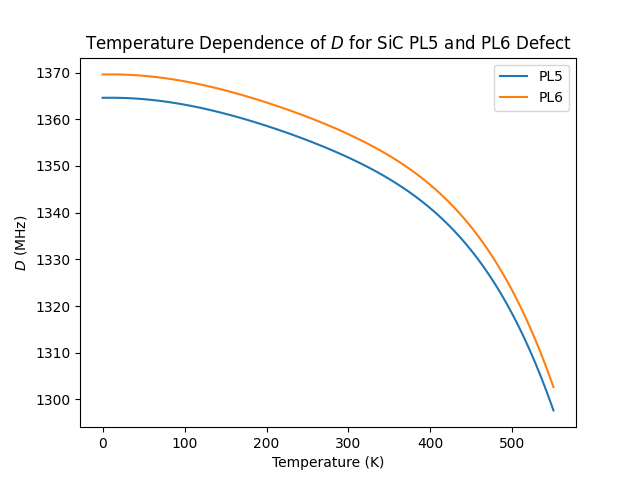
\includegraphics[width=0.49\textwidth]{figures/SiC-PL5PL6-D(T).png}
    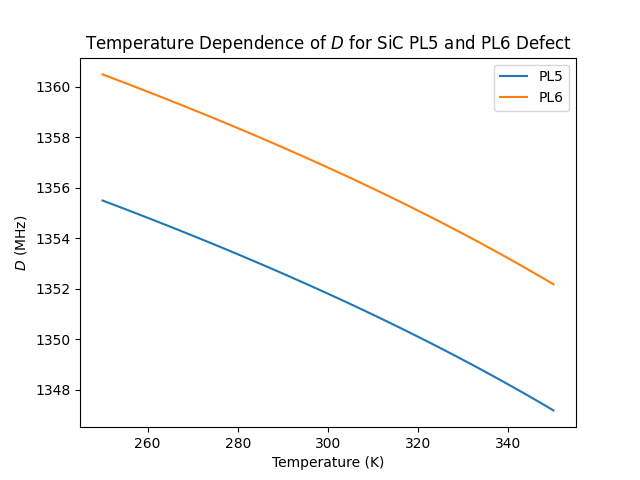
\includegraphics[width=0.49\textwidth]{figures/SiC-PL5PL6-D(T)-close.png}
    \caption{ZFS parameter $D$ temperature dependence for the PL5 and PL6 $S=1$ defect in SiC from 0-550 K (left) and 250-350 K (right). }\label{fig:PL5PL6DvsT}
\end{center}
\end{figure}

\td{Update the T dependence of PL5 and PL6 and regen the figure. Also update temp linear range in figure caption.}

In the simplest case thermometry is then achieved in the presence of a well known applied magnetic field. 

The measurement stems from the change of the value of
D mapped into the change of the oscillation frequency of the
relative variation of the photoluminescence intensity induced by the microwave pulse sequence.

Since the degeneracy is raised symmetrically, the value of $D$ is the average of the two resonant frequencies. The value of $D$ can then be mapped to a temperature. 

This is visualised in figure \ref{fig:pl6-3temps}. 

\begin{figure}[h]
    \begin{center}
        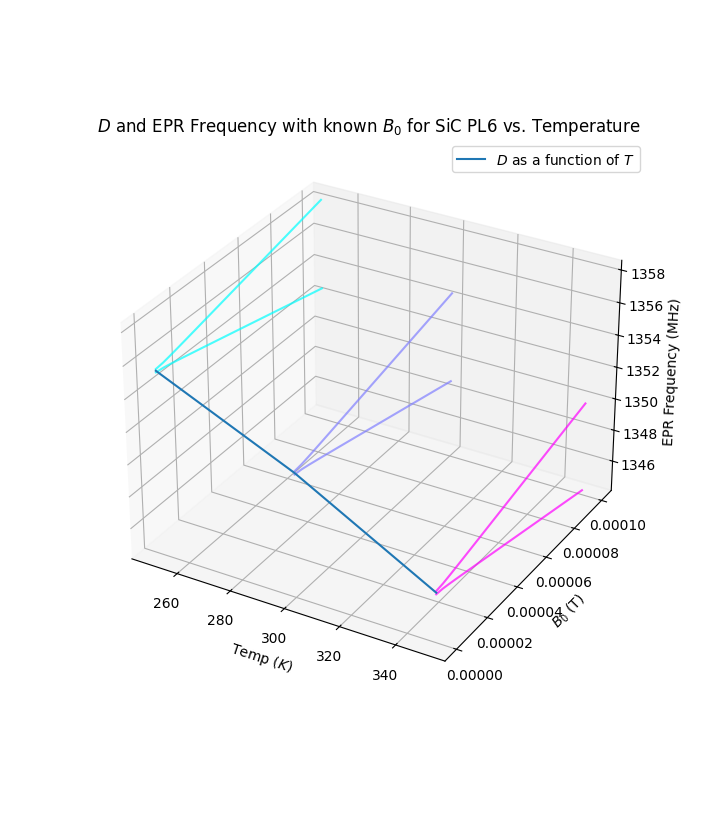
\includegraphics[width=0.8\textwidth]{figures/PL6-DvsT-3temps.png}
    \end{center}
    \caption{\td{write caption}}\label{fig:pl6-3temps}
\end{figure}

In practice this \td{Write up the Ramsey Interference methods for c-axis and basal from Castello p18}. 



\section{$S= 3/2$ Thermometry}\label{spin1.5-thermo}
% \todo[inline, color=ediblue]{Check wrapfigs}

We consider again the V2 Silicon vacancy which due to the 4H-SiC trigonal
pyramidal symmetry has a stable ground state ZFS with respect to temperature and can not be used for thermometry \cite{Castelletto_2024}.
% However, the ZFS of the excited state of the Silicon vacancy has a much
% larger change rate with the temperature compared with the
% dD/dT of the ground state of the divacancy in 4H-SiC or the
% NV centre in diamond \cite{Anisimov2016}.

% This can be a promising tool for
% thermometry, although the change of the ZFS of the excited
% state can not be detected directly from the ODMR spectrum
% due to the short lifetime of the excited state. As discussed
% in the magnetometry section, in the vicinity of the LAC, the
% PL intensity reaches a local extreme point [28]. By adding a
Schemas have been developed which exploit the increase in photoluminescence in the vicinity of level anti-crossings to measure the change in the excited state $D$ as in the work by Anisimov et al.

We will focus instead on an alternative all optical method which exploits the dependence on temperature of the photoluminescence of the spin system.

Anti-Stokes excitation is a process in which the wavelength of the exciting photon is longer (i.e. lower energy) than that
of the emitted photons (visualised in figure \ref{fig:anti-stokes}).  The mechanisms of anti-stokes excitation have been studied and include multiphoton absorption, phonon absorption, and Auger recombination
\cite{Tran2019, Wang2019}.

\begin{wrapfigure}{l}{0.37\textwidth}%
	\centering%
	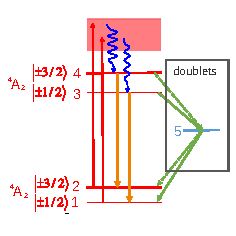
\includegraphics[width=0.37\textwidth]{figures/actual-stokes.pdf}
    \caption{Energy level diagram showing Stokes excitation. Colours as described in figure \ref{fig:big_stokes}. Adapted from Wang et al.}
    \label{fig:stokes}
	% \todo[inline, color=ediblue]{Write caption}
\end{wrapfigure}%



The anti-Stokes excitation process depends on a contribution from phonons (blue arrows in in figure \ref{fig:anti-stokes}).

By comparing the intensity of the anti-Stokes and Stokes photoluminescence we find the ratio between the intensities to be proportional to the phonon density, which are determined by a Bose–Einstenin distribution \cite{Wang2018}
\begin{equation}
	\frac{I_{\ce{AS}}}{I_{\ce{S}}} \propto \exp\left\{\frac{\Delta E}{k_B T} -1 \right\}
	\label{eq:anti-stoke-ratio}
\end{equation}
where $I_{\ce{AS}}$ and $I_{\ce{S}}$ represent respectively the intensities of the anti-Stokes and Stokes photoluminescence at a datum laser power. $\Delta E$ represents the difference in energy between the incident photon and the zero phonon line i.e. the phonon contribution to the excitation.

\begin{wrapfigure}{r}{0.4\textwidth}%
	\centering%
	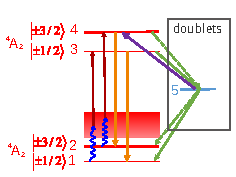
\includegraphics[width=0.4\textwidth]{figures/stokes.pdf}
    \caption{Energy level diagram showing anti-Stokes excitation. Colours as described in figure \ref{fig:big_stokes}. Adapted from Wang et al.}
    \label{fig:anti-stokes}
	% \todo[inline, color=ediblue]{Write caption}
\end{wrapfigure}%
% When ∆E ≫ kB T,
% we approximately have IASPL /IPL ∝ exp(−∆E/kB T) [165].

We may reduce this to a temperature dependent exponential curve when $\Delta E \ll k_B T$ as \eqref{eq:anti-stoke-ratio} reduces to
\begin{equation}
	\frac{I_{\ce{AS}}}{I_{\ce{S}}} \propto \exp\left\{\frac{\Delta E}{k_B T} \right\}.
	\label{eq:anti-stokes-ratio-reduced}
\end{equation}

Wang et al analysed the Silicon vacancy under anti-Stokes excitation \cite{Wang2021}. The zero phonon line for the defect is around $917$nm, so a Stokes excitation was induces by a laser with $1030 > 917$nm and the anti-Stokes excitation was induced by a laser with $720 < 917$nm. Using the same power for both lasers, the intensity of the photoluminescence from the anti-Stokes excitation increased as temperature increased. Conversely the intensity from the Stokes excitation decreased with temperature. The ratio therefore agrees with the statistical model in \eqref{eq:anti-stoke-ratio}.

Thus to realise a thermometer, we fit data to \eqref{eq:anti-stokes-ratio-reduced} with measurable proportionality and correction factors $a, b, c, T_0$ as \cite{Tran2019}
\begin{equation}
	\frac{I_{\ce{AS}}}{I_{\ce{S}}} = a +  b\exp\left\{-\frac{c}{T - T_0} \right\}.
	\label{eq:s1.5thermo_exponential}
\end{equation}

Temperature may then be inferred by solving the equation as
\begin{equation}
	T = T_0 - \frac{c}{\ln\left(\left[{\frac{I_{\ce{AS}}}{I_{\ce{S}}} - a}\right]/b\right)}.
	\label{eq:anti-stokes-solution}
\end{equation}

For the SiC Silicon vacancy the intensity ratio, and thus the proposed thermometry sensitivity, is most sensitive at room temperature and above.

This technique is also extremely versatile as the influence of external parameters, providing they do not change the position of the zero phonon line (effect ZFS $D$), does not affect the measurement. For example, figure \ref{fig:anti-stokes-ODMR} shows that the ODMR signature which can be used to detect magnetic field can be read in parallel to the ratio of intensities of the Stokes/anti-Stokes excitations. We will discuss how this may be applied in Chapter \ref{ch:results}.



\begin{figure}[h]
	\centering
	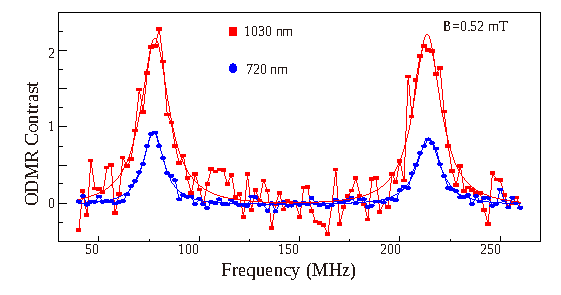
\includegraphics[width=0.8\textwidth]{figures/anti-stokes-ODMR.pdf}
	\caption{ODMR spectra for V2 Silicon vacancy using Stokes (blue) and anti-Stokes (red) excitation. This shows the Rabi frequencies are the same under either excitation scheme. Adapted from Wang et al}
    \label{fig:anti-stokes-ODMR}
	% Stokes
	% (blue) and AS excited (red) ODMR spectra of VSi defects for the same Rabi frequency (0.8 MHz) at different c-axis external magnetic fields
\end{figure}



% \todo[color=red, inline]{Affects of other factors? e.g. $\vec{B}, \vec{E}$}


% \begin{figure}[H]
%     \begin{center}
%         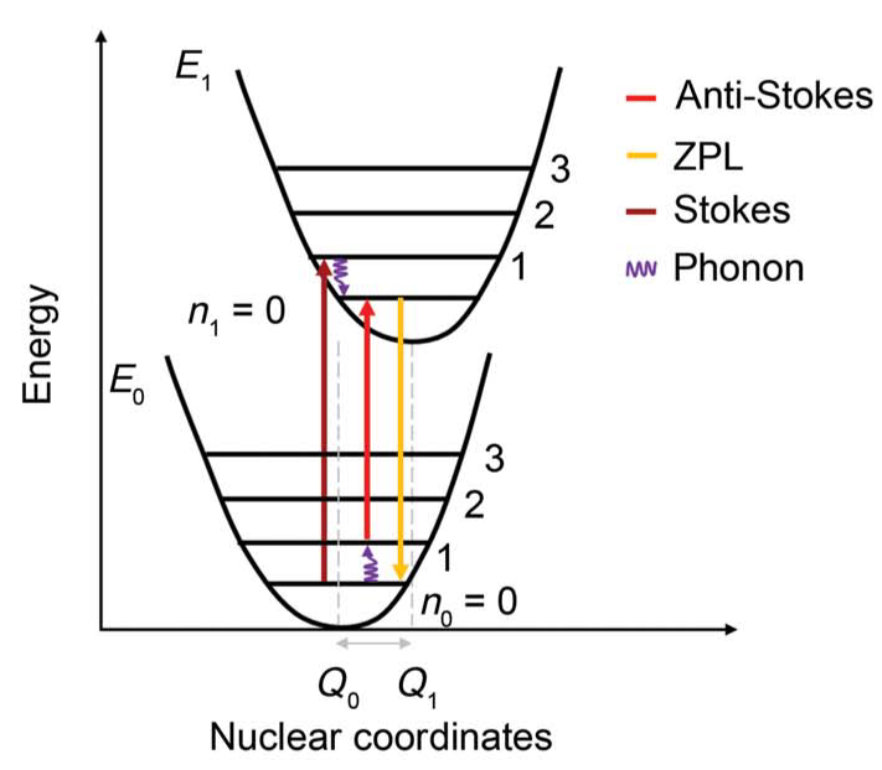
\includegraphics[width=0.4\textwidth]{figures/stokes.png}
%     \end{center}
%     \caption{}\label{fig:stokes}
% \end{figure}


\begin{summary}{$S=3/2$ Thermometry Summary}{sum:spin1.5thermo}
	We may achieve optical thermometry using an $S = 3/2$ system provided:
	\begin{enumerate}
		\item The ZFS parameters $D$ and $E$ are well known and we may determine the position of the zero phonon line.
		\item The system is responsive to both Stokes and anti-Stokes excitation and the intensities of the subsequent emission can be measured.
		\item The temperature dependence of the ratio between intensities has been studied and mapped to an exponential equation as             \begin{equation}
			      \tcbhighmath{
				      \frac{I_{\ce{AS}}}{I_{\ce{S}}} = a +  b\exp\left\{-\frac{c}{T - T_0} \right\},
			      }
			      \tag{\ref{eq:s1.5thermo_exponential}}
		      \end{equation}
		      from which the temperature can be calculated as
            \begin{equation}
			      \tcbhighmath{
				      T = T_0 - \frac{c}{\ln\left(\left[{\frac{I_{\ce{AS}}}{I_{\ce{S}}} - a}\right]/b\right)}.
			      }
			      \tag{\ref{eq:anti-stokes-solution}}
		      \end{equation}


	\end{enumerate}
\end{summary}




%%%%%%%%%%%%%%%%%%%%%%%%%%%%%%%%%%%%%%%%%%%%%%%%%%%%%%%%%%% TODO LINE %%%%%%%%%%%%%%%%%%%%%%%%%%%%%%%%%%%%%%%%%%%%%
% % \chapter{Multimodal Systems}

% \section{Multimodality}
% To develop our multimodal system we will start with a very simple model with the assumption that the applied $\vec{B}$ field is parallel to the defect axis. From there we will iterate our ensemble and work to reduce the number of assumptions.
%

\section{Proposed Systems}
We have described schemas for measuring the $\vec{E}$ field, $\vec{B}$ field, temperature, pressure and strain. We will say that the measurement of $T$ and $P$ should be considered equivalent in a $S=1$ system and the measurement of strain is equivalent to $\vec{E}$ in all systems.

Thus, we have $^4 C _2 = 6$ distinct pairwise combinations we may consider for multimodal application:
($\vec{B}$, $T$), ($\vec{B}$, $P$), ($\vec{B}$, $\vec{E}$), ($\vec{E}$, $T$), ($\vec{E}$, $P$) and ($T$, $P$).

We will discuss the combinations for which multi-modality is possible using the techniques described in this work.
% If not possible, we discuss why and if development of the literature could make such a sensor possible. 
Throughout the discussion, all external parameters not discussed are assumed to be absent.

% \subsection{$\vec{B}$ Multimode}
\subsection{$\vec{B}$ and Temperature}\label{sec:multimode_BT}
In general, simultaneously measuring $\vec{B}$ and $T$ is not possible as when the magnetic field is at $\theta \neq 90$, ZFS $D$ may not be inferred from the ODMR spectra. However, aligning $\vec{B}$ perpendicular to the defect axis allows $D$ to be calculated from the spectra and the magnitude of the field to be measured. 

\begin{proposal}{$|\vec{B}|$ and Temperature}
	We exploit the temperature independence of the V2 Silicon vacancy to measure the $\vec{B}$ field. Temperature may then be measured by either the same defect using anti-Stokes technique or a divacancy where temperature may be inferred from the change in ZFS $D$.
\end{proposal}
\begin{figure}[h]
	\begin{center}
		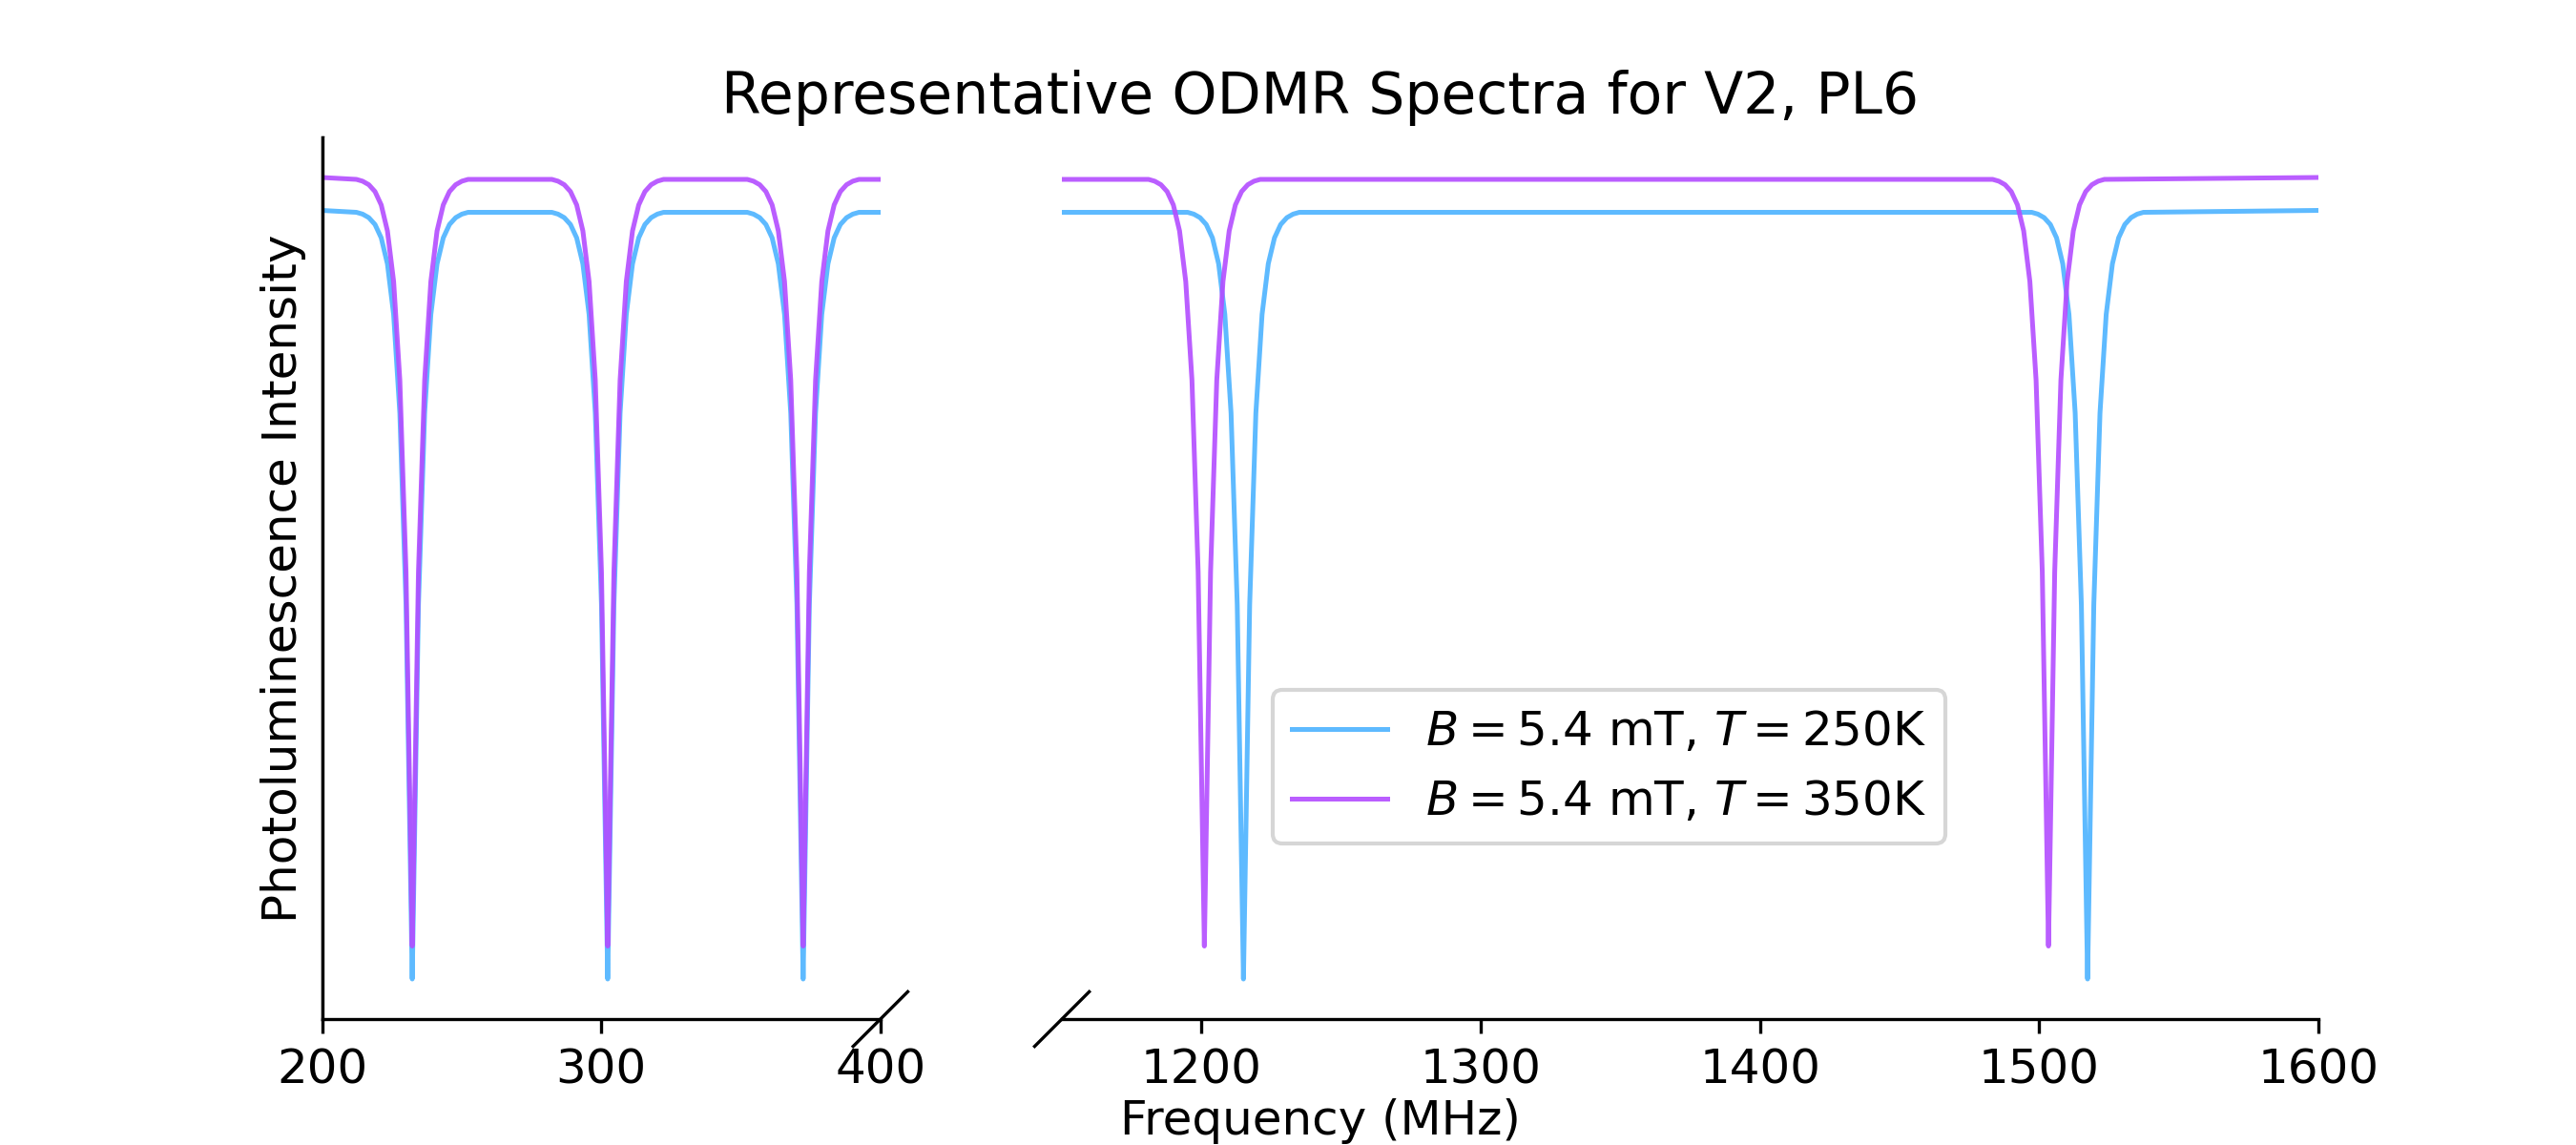
\includegraphics[width=0.95\textwidth]{figures/ODMR-multimodal-s15magnet-s1T.png}
	\end{center}
	\caption{Representative ODMR spectra for an ensemble of PL6 and V2 defects showing the shift in ZFS $D$ due to temperature in the PL6 and lack of shift in the V2. Dashed lines indicate the position of $D$ for the PL6 defect. }
    \label{fig:multimode_BT}
    % \todo[inline, color=ediblue]{Write caption}
\end{figure}
The implementation is to capture the ODMR spectra of the defects. Figure \ref{fig:multimode_BT} shows a two simulated spectra for a V2 and PL6 ensemble at 250K and 350K (offset for clarity). Clearly the V2 spectra is unaffected by temperature allowing $\vec{B}$ to be measured from the three frequencies as described in summary \ref{sum:spin1.5magnet}. Providing the ZFS $D$ of the PL6 is under no other influence e.g. pressure or $\vec{E}_\parallel$, $D(T)$ may be read from the two frequencies of the PL6 defect as described in \ref{sum:spin1thermo}.





\subsection{$\vec{B}$ and Pressure}
As for \ref{sec:multimode_BT} this is not possible in general and required $\vec{B}$ to be perpendicular to the defect axis. 

\begin{proposal}{$|\vec{B}$| and Pressure}
	We exploit the linear dependence of the V2 Silicon vacancy $D$ and pressure, and the linear dependence on $\Delta f$ of the divacancy on the applied $\vec{B}$ field. We determine the pressure from the average of the two EPR frequencies for the divacancy and use the inferred pressure to perform magnetometry. 

\end{proposal}

\begin{figure}[h]
	\begin{center}
		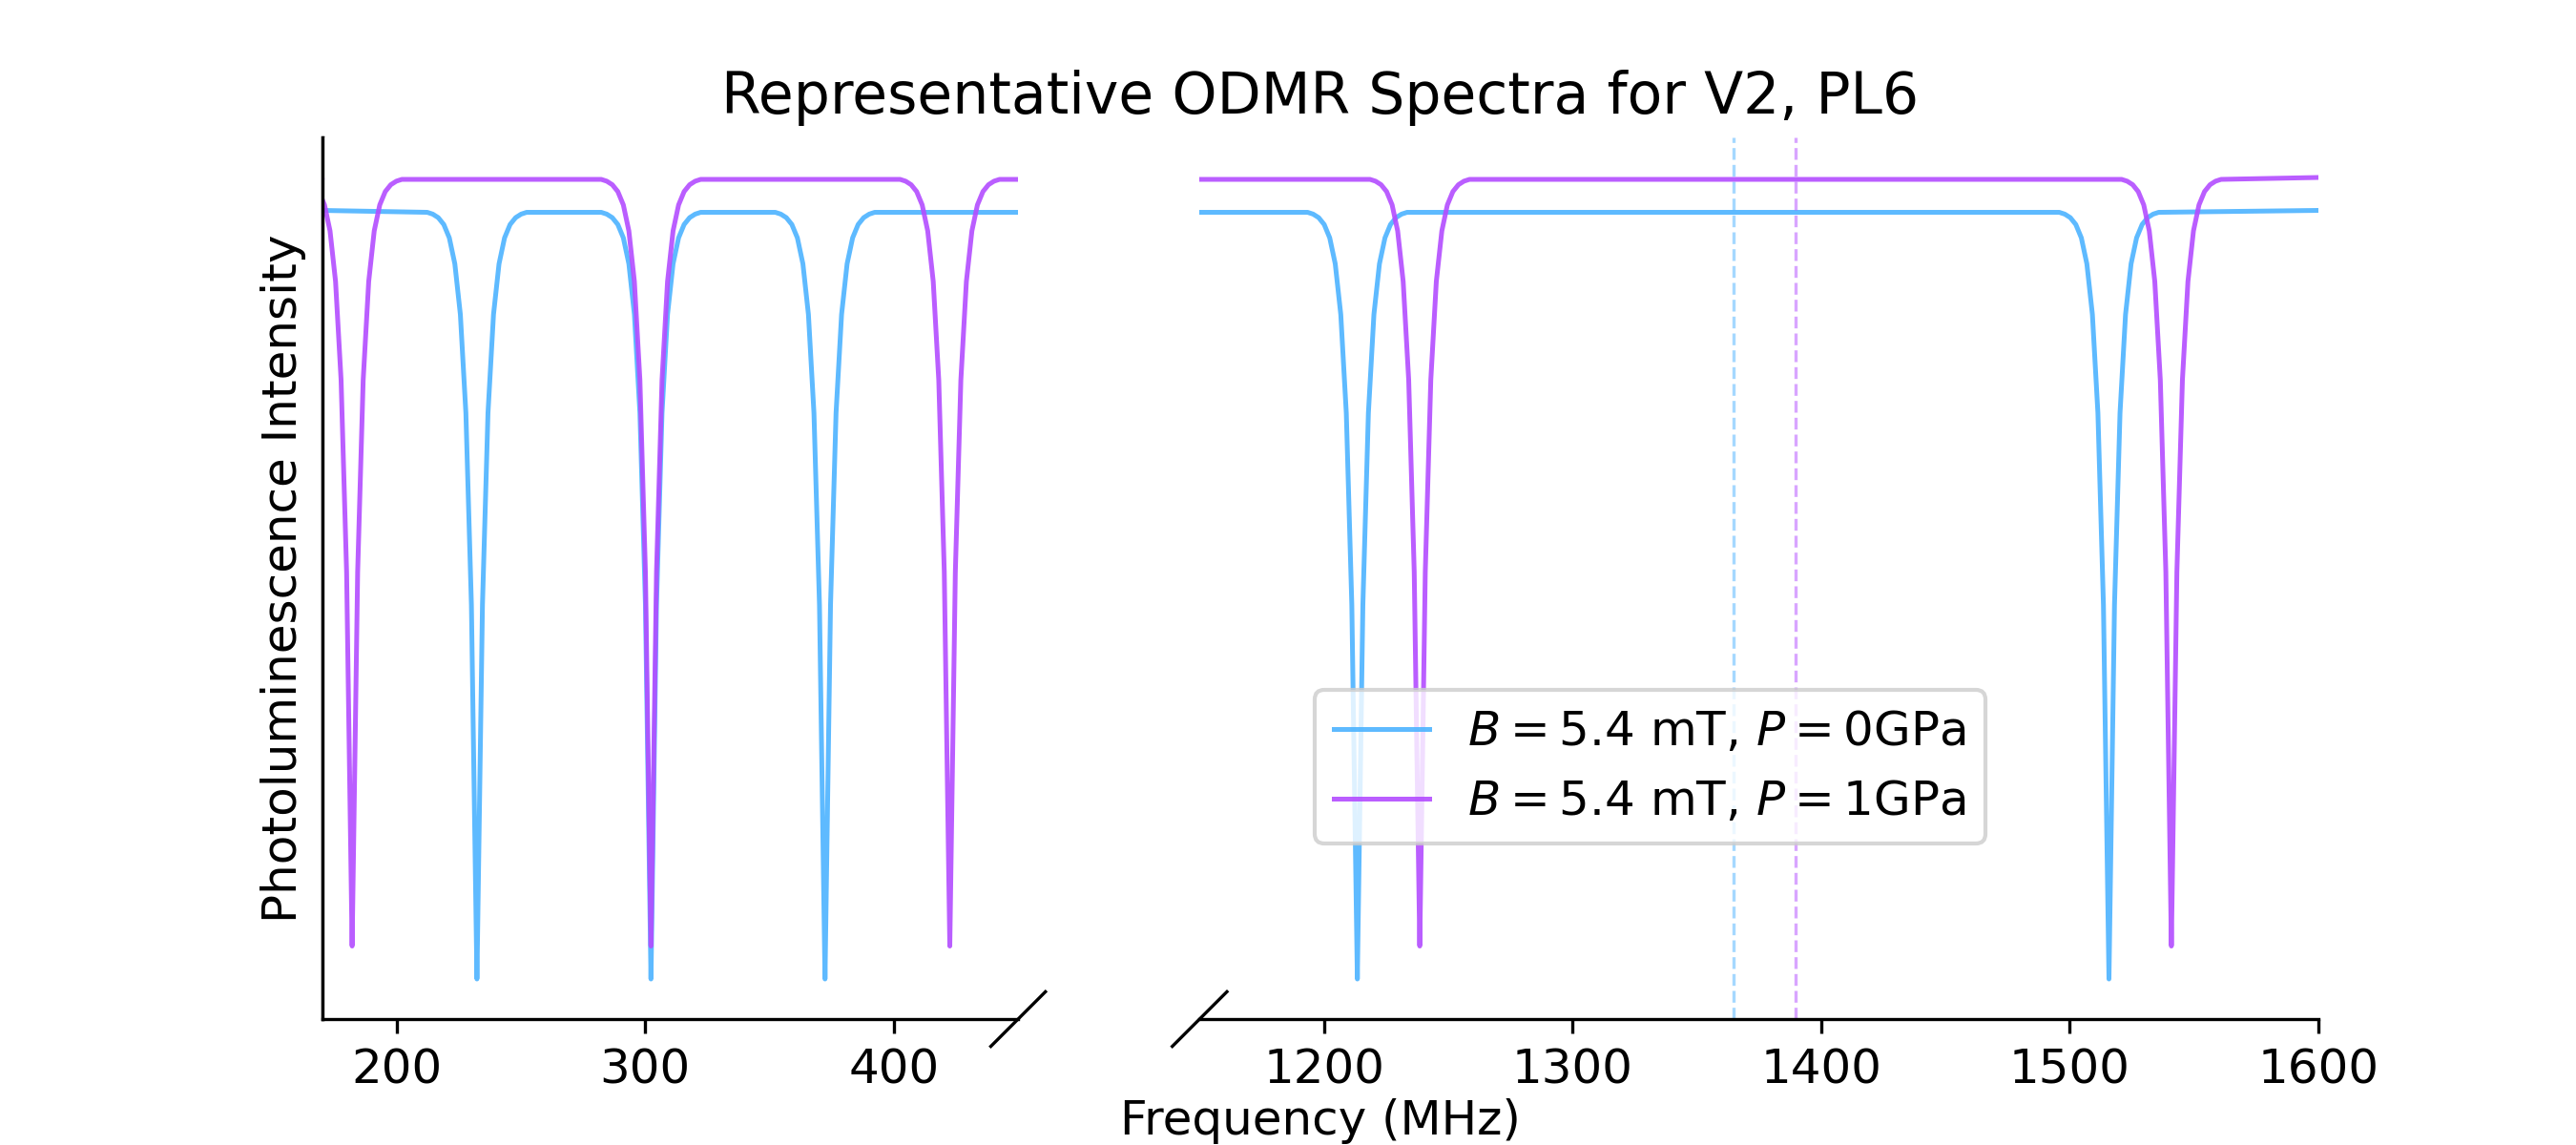
\includegraphics[width=0.95\textwidth]{figures/ODMR-multimodal-s15magnet-s1P.png}
	\end{center}
	\caption{Representative ODMR spectra for an ensemble of PL6 and V2 defects showing the shift in ZFS $D$ of both the PL6 and V2 defect due to applied pressure. Dashed lines indicate the position of $D$ for the PL6 defect.}
    \label{fig:multimode_BP}
    % \todo[inline, color=ediblue]{Write caption}
\end{figure}

The approach is slightly less straight forward as the ZFS $D$ of the Silicon vacancy shows a linear dependence on $P$. Thus, we cannot cleanly separate the two parameters as above. However, since the dependence is linear, as is the dependence of an $S=1$ defect splitting on the $\vec{B}$ field, and the $B$ field does not influence $D$, we may still determine the parameters simultaneously.

The implementation is to first measure $D(P)$ by taking the average of the two frequencies of the $S=1$ defect (\ref{sum:spin1.5thermo}). Now the pressure is known, calculate $D(P)$ for the Silicon vacancy and perform magnetometry with the V2 Silicon vacancy as detailed in \ref{sum:spin1.5magnet}.


\subsection{Temperature and Pressure}\label{multi_TP}
Simultaneously measuring temperature and pressure
% is not currently possible due to a lack of understanding of the interplay between $T$ and $P$ and the combined effect on $D$.
may be achieved using only the V2 Silicon vacancy. Illustrative ODMR plots are shown with $\vec{B}$ applied parallel to the defect axis. 

\begin{proposal}{Temperature and Pressure}
    The temperature independence of the V2 Silicon vacancy allows the CW-ODMR spectra to be inspected to evaluate $P$ from $D(P)$. 
    With knowledge of the effective $D$, tune two lasers to a Stokes and anti-Stokes frequency and perform $S=3/2$ temperature measurements. 
\end{proposal}


The ODMR spectra of the V2 Silicon vacancy in zero field (magnetic or electric) will show a single peak at the effective $D$. 
This may be used to determine the position of the zero phonon line from which temperature measurement can be performed as described in \ref{sum:spin1.5thermo}. 

\begin{figure}[h]
    \begin{center}
        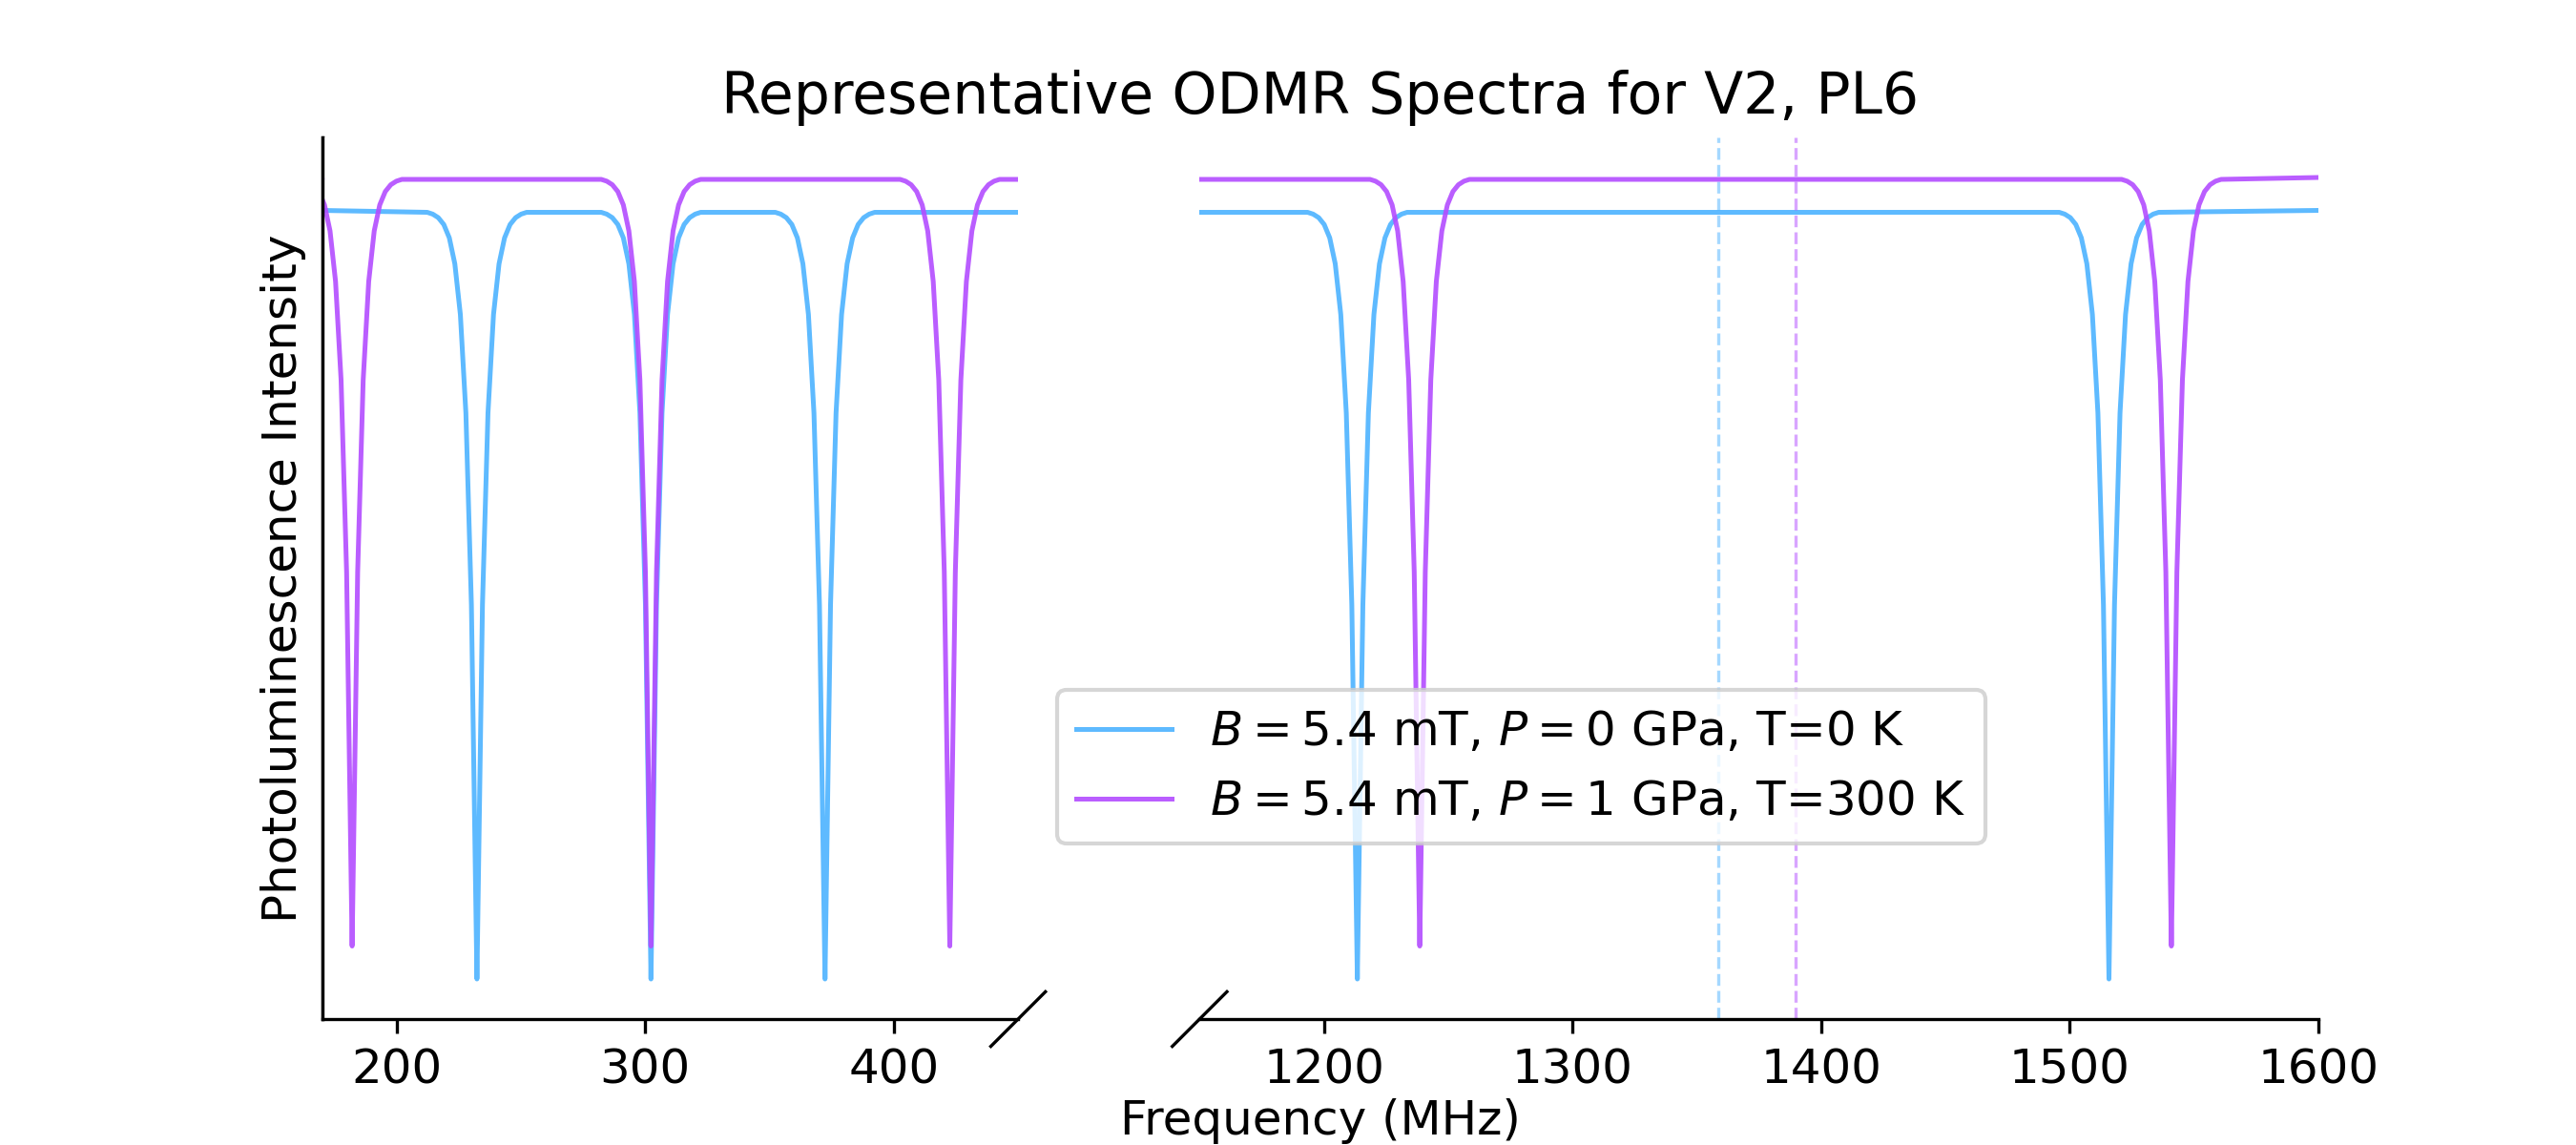
\includegraphics[width=0.95\textwidth]{figures/ODMR-multimodal-s15magnet-s1PT.png}
    \end{center}
    \caption{Representative ODMR spectra for an ensemble of PL6 and V2 defects showing the inequivalent shifting of ZFS $D$ due to pressure and temperature assuming the effects compound additively. Dashed lines indicate the position of $D$ for the PL6 defect.}
    \label{fig:multi-TP}
    % \todo[inline, color=ediblue]{Write caption}
\end{figure}


% Theoretically, the measurement may be simultaneously completed using only the V2 Silicon vacancy, but temperature sensing using the 

% However, since for the V2 Silicon vacancy $D$ is not dependent on $T$ but linearly dependent on $P$, the pressure may be isolated by studying the spectra of that defect.

In practice, readily tuning lasers to respond to the effective $D$ may be impractical. If future work mapped a function $D(P,T)$ for the divacancy, it could be used to perform temperature measurement using only CW-ODMR techniques. 

To demonstrate, we (naively) assume the effects of temperature and pressure on the ZFS $D$ of the divacancy linearly combine, we visualise this in figure \ref{fig:multi-TP}. 

If all three frequencies are visible ($f_1 < f_2 < f_3$) in the $S=3/2$ spectra we see using \eqref{eq:spin1.5_magnet_Bparallel_eigenvalues} that we may determine $D$ using 
\begin{equation}
    D(P) = \frac{f_1 -f_3 }{4},
    \label{eq:}
\end{equation}
from which we infer the pressure $P_0$ as no dependence on $T$ is shown.     

We now fit the data to compute $T$ in the using the divacancy frequencies ($\nu_1, \nu_2$) as 
\begin{equation}
    D(T, P_0) = \frac{\nu_2 + \nu_1}{2}.
    \label{eq:}
\end{equation}
% this could be reduced by substitution of the measured pressure in the V2 defect ($P_0$), and a fit to the divacancy spectra of $D(P_0, T)$, from which we would determine $T$.

% \subsection{$\vec{E}$ Multimode}
\subsection{$\vec{E}$ and Temperature or Pressure}\label{multi-E-pressure}
The measurement of $\vec{E}$ in parallel to temperature (pressure) is less clear, as the influence of $E_\parallel$ is indistinguishable from a change in temperature (pressure) - a net change in ZFS $D$. Ideally, we would exploit the temperature independence of the V2 defect $D$ but we have been unable to find a schema for $S=3/2$ electrometry. 
Thus, within the context of this work we have been unable to find a scheme to simultaneously measure $\vec{E}$ and temperature (pressure) in general.  

An exception can be made however if careful alignment of the $\vec{E}$ is possible, then the magnitude may be measured. 

\begin{proposal}{$|\vec{E}|$ and Temperature (Pressure)}
    The $\vec{E}$ field is aligned perpendicular to the defect axis. Then by \eqref{eq:s1_elect_perp} we may determine the magnitude with no dependence on $D$. With knowledge of the $|\vec{E}|$, choose a defect on the same axis and calculate the influence of $\vec{E}$ on $D$ and $E$. Measure $D(\vec{E}, T)$ and fit the data to calculate the temperature (pressure) of the system. 
\end{proposal}

We infer from the electrometry Hamiltonian \eqref{eq:electometry_matrix_hamiltonian} that the corrections to $D$ and $E$ are 
\begin{equation}
    \Delta D = d_\parallel |\vec{E}| \cos\theta_E, \quad \Delta E = d_\perp |\vec{E}| \sin \theta_E.
    \label{eq:}
\end{equation}

We exploit that when $\theta = 90^\circ$ the ZFS $D$ is not affected by the field and any variation must be due to temperature (pressure). 

In the absence of an applied magnetic field (which would have to of known magnitude and applied parallel to the defect axis for this schema to work), $E$ is determined from the effective magnitude of ZFS $E$ by the difference in the frequencies as
\begin{equation}
    E_\perp d_\perp = E_0 - \sqrt{\frac{(f_1 - f_2)^2}{4} - (g \mu_B B)^2}, 
    \label{eq:multi-E+T}
\end{equation}
where $E_0$ is the ZFS $E$ of the defect without influence of the electric field. 

Temperature (pressure) sensing can also then be performed using the same two measured frequencies as $D(T)$ will be the average of them. 

Figure \ref{fig:E_Field_perp_temp} which shows a strictly perpendicular electric field allows a visualisation of the described effects.  
\begin{figure}[H]
    \begin{center}
        % 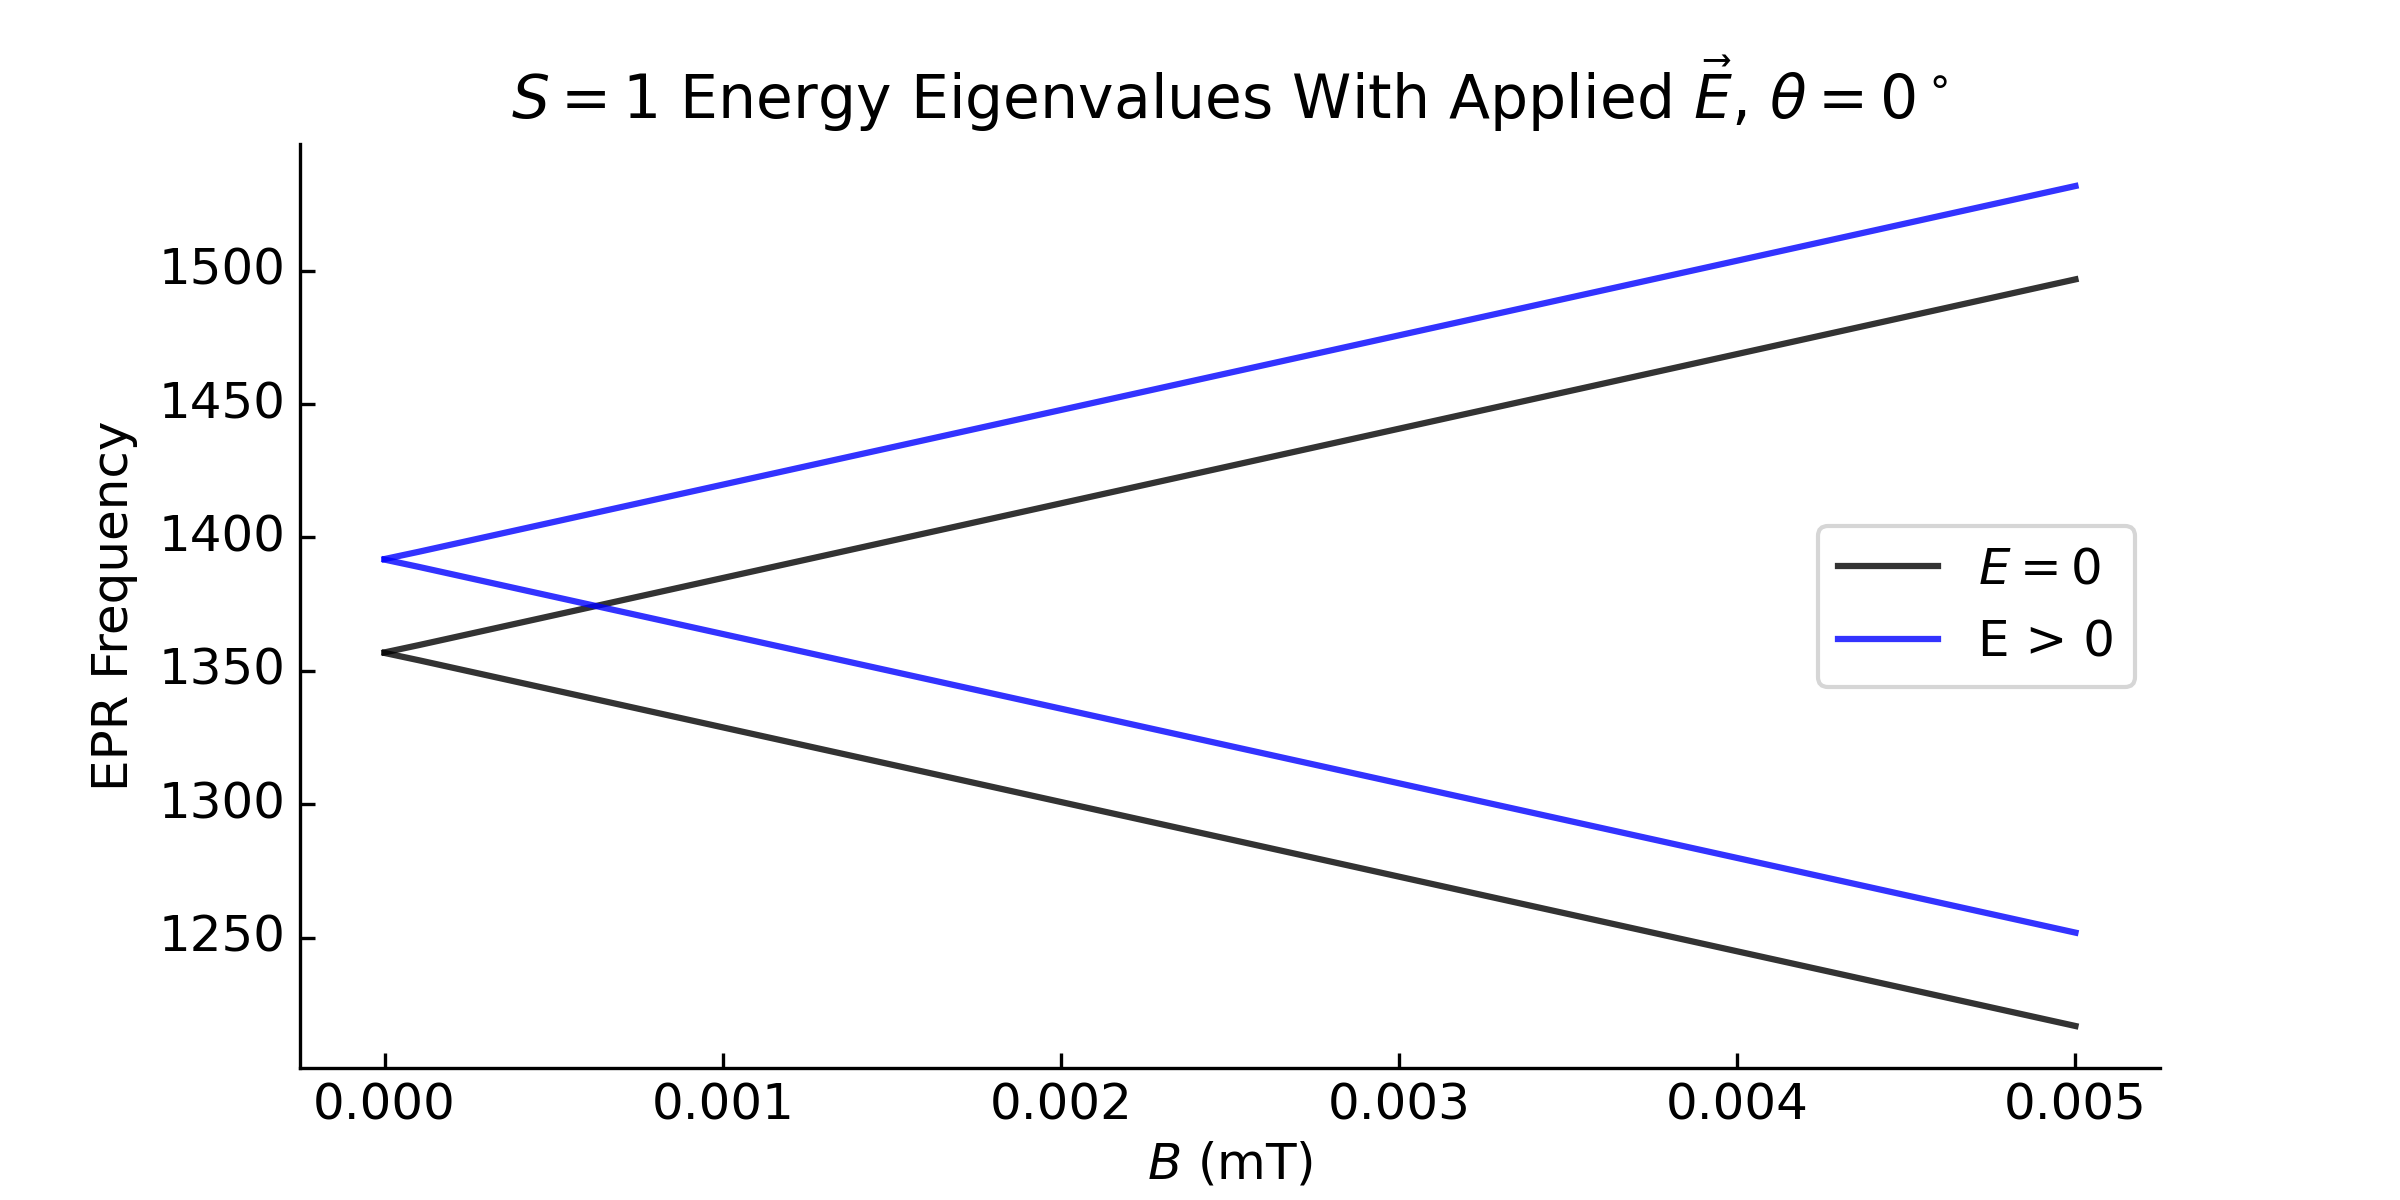
\includegraphics[width=0.95\textwidth]{figures/EFieldParallel.png}
        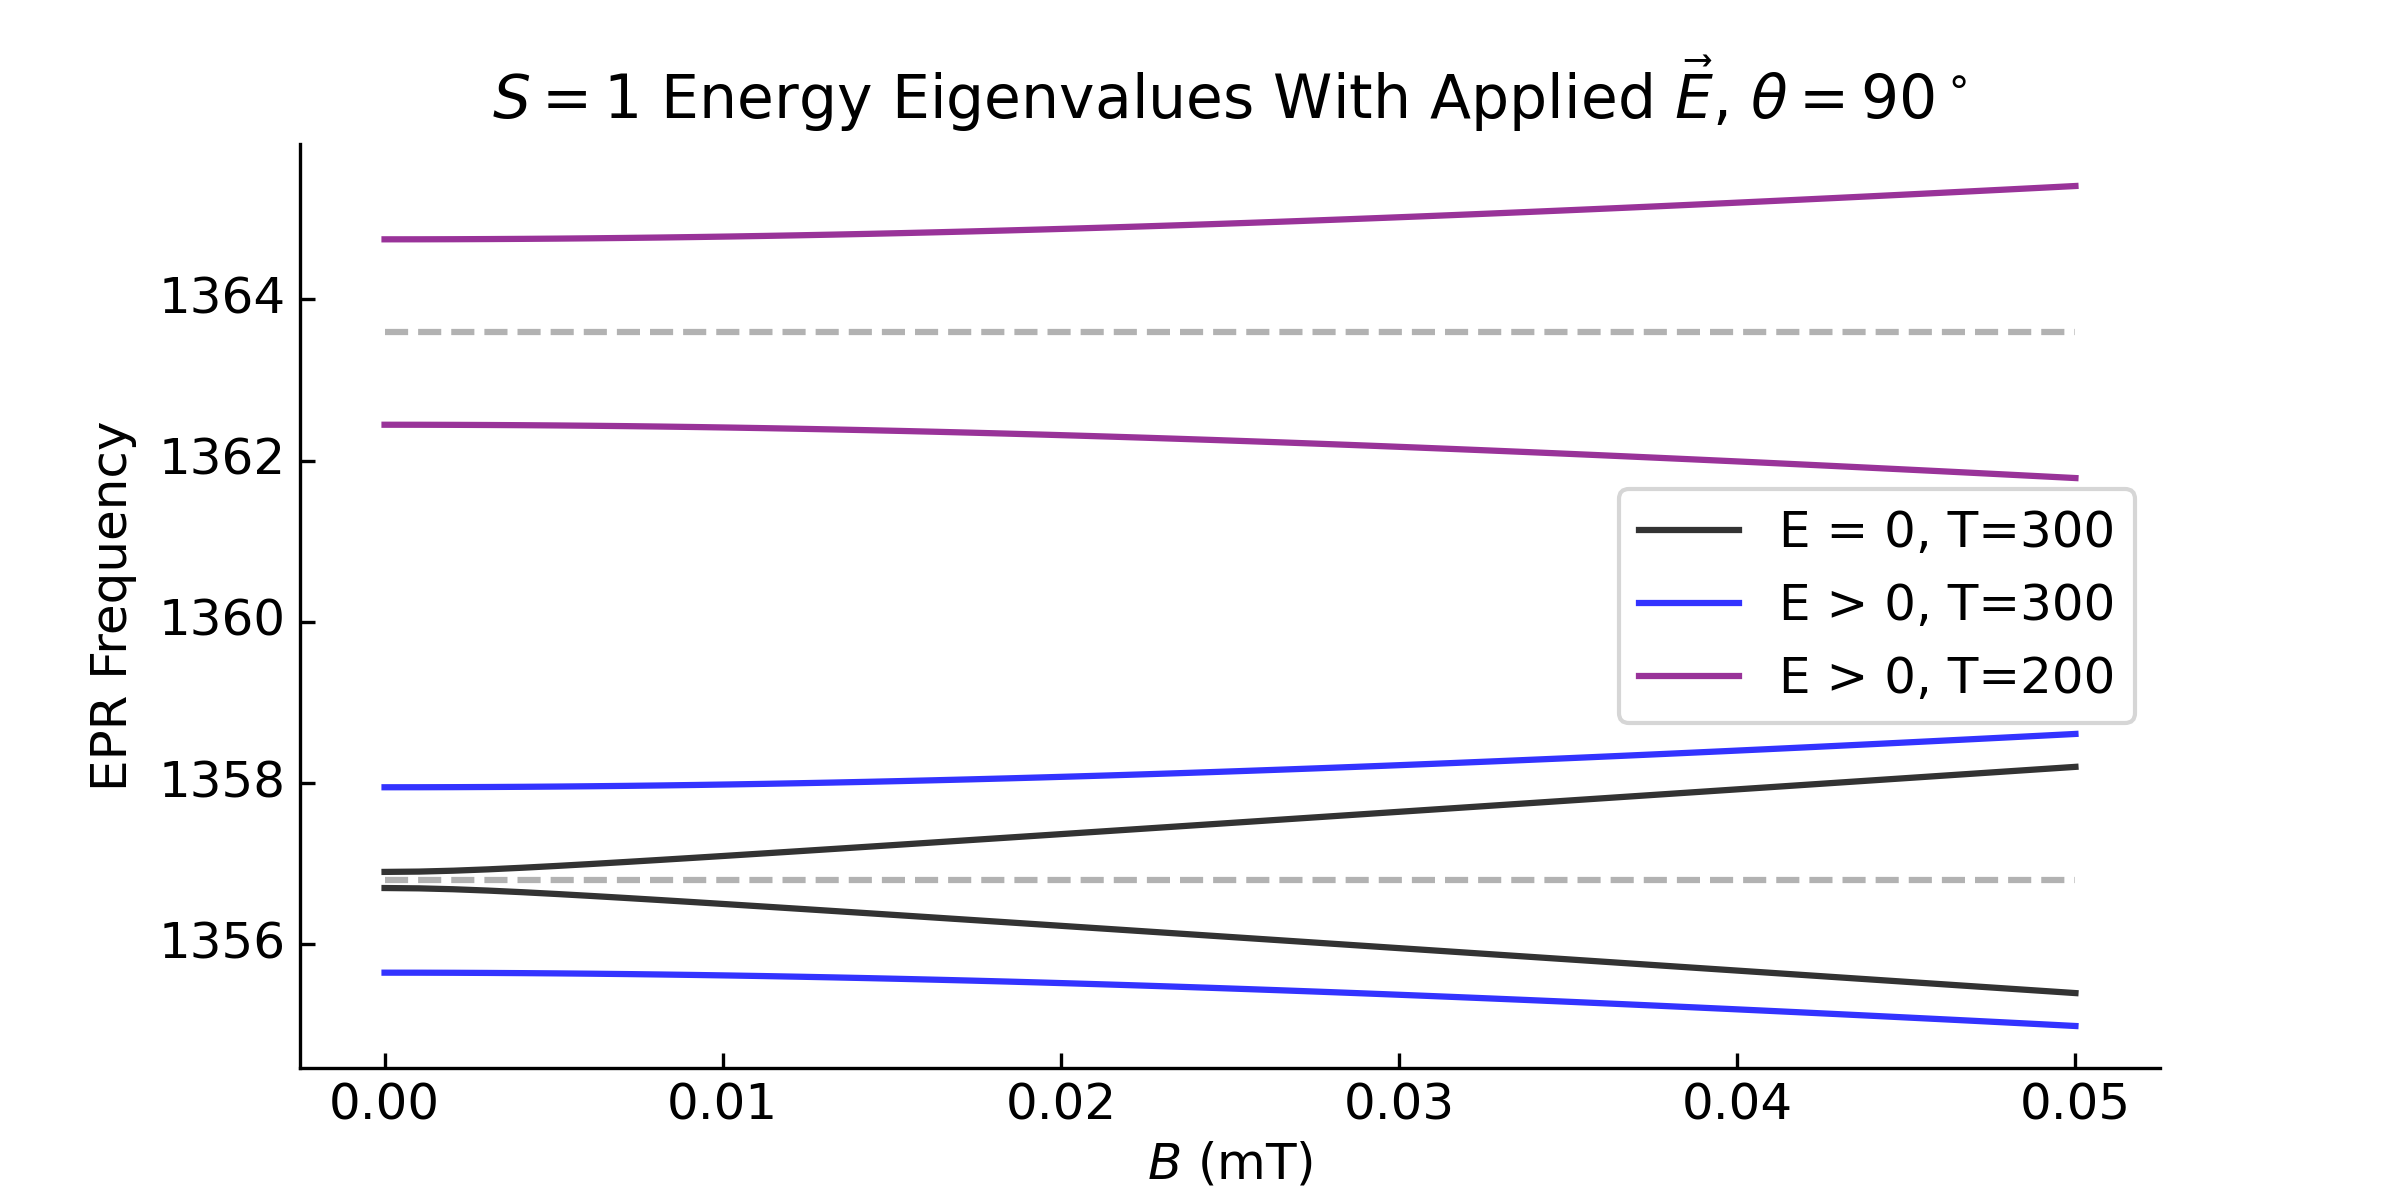
\includegraphics[width=0.95\textwidth]{figures/EFieldPerpTemp.png}
        % \missingfigure{ODMR/Energy plot showing effect of parallel/perp E field}
    \end{center}
    \caption{Eigenvalue plot showing that ZFS $D$ (dashed line) is the average of the two measured frequencies at a given temperature, parallel $\vec{B}$ field and perpendicular $\vec{E}$ field.}\label{fig:E_Field_perp_temp}
    % \todo[inline, color=ediblue]{Write caption}
\end{figure}

% \subsection{Scalar Sensing}

% Using a similar scheme to that described above...

\subsection{Trimodal $\vec{B}$, Temperature and Pressure}
% If we assume the interplay and dependence of temperature and pressure on the ZFS $D$ are well understood for the Silicon vacancy and the divacancy, then a trimodal schema is possible. 

\begin{proposal}{$\vec{B}$, Temperature and Pressure}
    We exploit the temperature independence of the V2 Silicon vacancy to perform a pressure measurement. Then, having fixed $P_0$, we infer $T$. Now, since $T$ and $P$ are well known, we may perform scalar magnetometry using either the $S=1$ or $S=3/2$ defects provided the magnetic field is aligned parallel to the defect axis. 
\end{proposal}

This method simply extends the method described in \ref{multi_TP}. By fixing the orientation of the field, the magnitude of the field may be computed from either the $S=1$ or $S=3/2$ spectra respectively as 
\begin{equation}
    B = \frac{\nu_2 - \nu_1}{2 g\mu_B }, \quad B = \frac{f_3 + f_1}{2 g \mu_B } = \frac{f_2}{g \mu_B}.  
    \label{eq:}
\end{equation}

% The only regime in which the magnitude of both fields may be simultaneously determined is identical to that described above in \ref{multi-E-pressure}. The discussion may be extended by measuring the magnitude of the magnetic field using \eqref{eq:s1_parallel_magnetometry} and substituting it into \eqref{eq:multi-E+T} to find 
% \begin{equation}
%     E_\perp d_\perp = E_0 - \sqrt{\frac{(f_1 - f_2)^2}{4} - (g \mu_B B)^2}, 
%     \label{eq:multi-E+T2}
% \end{equation}
%
%
% \subsection{Tri-modality}\label{sec:trimodal}
% The success of \ref{sec:multimode_BT} and possible encapsulation into a single defect type allowed for the consideration of a trimodal sensor.
%
% \begin{proposal}{$\vec{B}$, $\vec{E}$ and Temperature}
% 	The PL6 defect acts solely as a electrometer. We consider the influence of $\vec{B}$ and $T$ to be well known and extracted from V2 Silicon vacancy.
% \end{proposal}
%





% \subsection{$|\vec{B}|$ and $T$}
% \cite{Degen2008}
%
% \subsection{Angle Resolved $|\vec{B}|$ and $T$}
% % We show that uniaxial color centers in silicon carbide with hexagonal lattice structure can be used to measure not only the strength but also the polar angle of the external magnetic field with respect to the defect axis with high precision. 
% \cite{PhysRevApplied.4.014009}
%
% \subsection{$\vec{B}$ and $T$}
%
%
% \subsection{$|\vec{B}|$, $|\vec{E}|$ and $T$}
% The influence of an $\vec{E}$ field parallel to the defect axis is indistinguishable from the influence of a change of temperature. Similarly, the influence of an $\vec{E}$ field perpendicular to the defect axis is indistinguishable from the influence of a $\vec{B}$ field parallel to the defect axis. The exception is when \td{When $B_0$ is smaller than ZFS E when the effects can be distinguished}...
%
% \begin{figure}[H]
% 	\begin{center}
% 		% \includegraphics[width=0.95\textwidth]{figures/}
% 		\missingfigure{2 plots. Both of a basline energy graph and showing the similarity of T and parallel E, and B and perp E.}
% 	\end{center}
% 	\caption{\td{write caption}}\label{fig:}
% \end{figure}
%
%
% Thus, to extend the multi-modality to include the $\vec{E}$ field we must isolate the influence of the $\vec{E}$ field from the other environmental factors.
%
%
%
% \subsection{$\vec{B}$, $\vec{E}$ and $T$}
%
%
% % \begin{summary}{Multimodality Summary}{sum:multimodal}
% % 	From the construction of our multimodal systems we have learned
% % 	\begin{enumerate}
% % 		\item The Silicon vacancy is resistant to temperature fluctuations so can be used to measure $\vec{B}$ \textbf{or} $\vec{E}$ while a divacancy monitors temperature.
% % 	\end{enumerate}
% % \end{summary}
% %
%%%%%%%%%%%%%%%%%%%%%%%%%%%%%%%%%%%%%%%%%%%%%%%%%%%%%%%%%%%%%%%%%%%%%%%%%%%%%%%%%%%%%%%%%%%%%%%%%%%%%%%%%%%%%%%%%%%%%%%%%%%55

% \subsection{$\vec{B}$ and $\vec{E}$}
% Even more difficult is the separation of $\vec{B}$ and $\vec{E}$. 
% Using the techniques in this work no general solution was found for simultaneously measuring both fields.


%%%%%%%%%%%%%%%%%%%%%%%%%%%%%%%%%%%%%%%%%%%%%%%%%%%%%%%%%%%%%%%%%%%%%%%%%%%%%%%%%%%%%%%%%%%%%%%%%%%%%%%%%%%%%%%%%%%%
